% Options for packages loaded elsewhere
\PassOptionsToPackage{unicode}{hyperref}
\PassOptionsToPackage{hyphens}{url}
\PassOptionsToPackage{dvipsnames,svgnames,x11names}{xcolor}
%
\documentclass[
default
]{sn-jnl}

\usepackage{amsmath,amssymb}
\usepackage{iftex}
\ifPDFTeX
  \usepackage[T1]{fontenc}
  \usepackage[utf8]{inputenc}
  \usepackage{textcomp} % provide euro and other symbols
\else % if luatex or xetex
  \usepackage{unicode-math}
  \defaultfontfeatures{Scale=MatchLowercase}
  \defaultfontfeatures[\rmfamily]{Ligatures=TeX,Scale=1}
\fi
\usepackage{lmodern}
\ifPDFTeX\else  
    % xetex/luatex font selection
\fi
% Use upquote if available, for straight quotes in verbatim environments
\IfFileExists{upquote.sty}{\usepackage{upquote}}{}
\IfFileExists{microtype.sty}{% use microtype if available
  \usepackage[]{microtype}
  \UseMicrotypeSet[protrusion]{basicmath} % disable protrusion for tt fonts
}{}
\makeatletter
\@ifundefined{KOMAClassName}{% if non-KOMA class
  \IfFileExists{parskip.sty}{%
    \usepackage{parskip}
  }{% else
    \setlength{\parindent}{0pt}
    \setlength{\parskip}{6pt plus 2pt minus 1pt}}
}{% if KOMA class
  \KOMAoptions{parskip=half}}
\makeatother
\usepackage{xcolor}
\setlength{\emergencystretch}{3em} % prevent overfull lines
\setcounter{secnumdepth}{-\maxdimen} % remove section numbering
% Make \paragraph and \subparagraph free-standing
\ifx\paragraph\undefined\else
  \let\oldparagraph\paragraph
  \renewcommand{\paragraph}[1]{\oldparagraph{#1}\mbox{}}
\fi
\ifx\subparagraph\undefined\else
  \let\oldsubparagraph\subparagraph
  \renewcommand{\subparagraph}[1]{\oldsubparagraph{#1}\mbox{}}
\fi


\providecommand{\tightlist}{%
  \setlength{\itemsep}{0pt}\setlength{\parskip}{0pt}}\usepackage{longtable,booktabs,array}
\usepackage{calc} % for calculating minipage widths
% Correct order of tables after \paragraph or \subparagraph
\usepackage{etoolbox}
\makeatletter
\patchcmd\longtable{\par}{\if@noskipsec\mbox{}\fi\par}{}{}
\makeatother
% Allow footnotes in longtable head/foot
\IfFileExists{footnotehyper.sty}{\usepackage{footnotehyper}}{\usepackage{footnote}}
\makesavenoteenv{longtable}
\usepackage{graphicx}
\makeatletter
\def\maxwidth{\ifdim\Gin@nat@width>\linewidth\linewidth\else\Gin@nat@width\fi}
\def\maxheight{\ifdim\Gin@nat@height>\textheight\textheight\else\Gin@nat@height\fi}
\makeatother
% Scale images if necessary, so that they will not overflow the page
% margins by default, and it is still possible to overwrite the defaults
% using explicit options in \includegraphics[width, height, ...]{}
\setkeys{Gin}{width=\maxwidth,height=\maxheight,keepaspectratio}
% Set default figure placement to htbp
\makeatletter
\def\fps@figure{htbp}
\makeatother
% definitions for citeproc citations
\NewDocumentCommand\citeproctext{}{}
\NewDocumentCommand\citeproc{mm}{%
  \begingroup\def\citeproctext{#2}\cite{#1}\endgroup}
\makeatletter
 % allow citations to break across lines
 \let\@cite@ofmt\@firstofone
 % avoid brackets around text for \cite:
 \def\@biblabel#1{}
 \def\@cite#1#2{{#1\if@tempswa , #2\fi}}
\makeatother
\newlength{\cslhangindent}
\setlength{\cslhangindent}{1.5em}
\newlength{\csllabelwidth}
\setlength{\csllabelwidth}{3em}
\newenvironment{CSLReferences}[2] % #1 hanging-indent, #2 entry-spacing
 {\begin{list}{}{%
  \setlength{\itemindent}{0pt}
  \setlength{\leftmargin}{0pt}
  \setlength{\parsep}{0pt}
  % turn on hanging indent if param 1 is 1
  \ifodd #1
   \setlength{\leftmargin}{\cslhangindent}
   \setlength{\itemindent}{-1\cslhangindent}
  \fi
  % set entry spacing
  \setlength{\itemsep}{#2\baselineskip}}}
 {\end{list}}
\usepackage{calc}
\newcommand{\CSLBlock}[1]{\hfill\break\parbox[t]{\linewidth}{\strut\ignorespaces#1\strut}}
\newcommand{\CSLLeftMargin}[1]{\parbox[t]{\csllabelwidth}{\strut#1\strut}}
\newcommand{\CSLRightInline}[1]{\parbox[t]{\linewidth - \csllabelwidth}{\strut#1\strut}}
\newcommand{\CSLIndent}[1]{\hspace{\cslhangindent}#1}

%%%% Standard Packages

\usepackage{graphicx}%
\usepackage{multirow}%
\usepackage{amsmath,amssymb,amsfonts}%
\usepackage{amsthm}%
\usepackage{mathrsfs}%
\usepackage[title]{appendix}%
\usepackage{xcolor}%
\usepackage{textcomp}%
\usepackage{manyfoot}%
\usepackage{booktabs}%
\usepackage{algorithm}%
\usepackage{algorithmicx}%
\usepackage{algpseudocode}%
\usepackage{listings}%

%%%%

\raggedbottom
\usepackage{fontspec}
\usepackage{multirow}
\usepackage{multicol}
\usepackage{colortbl}
\usepackage{hhline}
\newlength\Oldarrayrulewidth
\newlength\Oldtabcolsep
\usepackage{longtable}
\usepackage{array}
\usepackage{hyperref}
\usepackage{float}
\usepackage{wrapfig}
\makeatletter
\@ifpackageloaded{caption}{}{\usepackage{caption}}
\AtBeginDocument{%
\ifdefined\contentsname
  \renewcommand*\contentsname{Table of contents}
\else
  \newcommand\contentsname{Table of contents}
\fi
\ifdefined\listfigurename
  \renewcommand*\listfigurename{List of Figures}
\else
  \newcommand\listfigurename{List of Figures}
\fi
\ifdefined\listtablename
  \renewcommand*\listtablename{List of Tables}
\else
  \newcommand\listtablename{List of Tables}
\fi
\ifdefined\figurename
  \renewcommand*\figurename{Figure}
\else
  \newcommand\figurename{Figure}
\fi
\ifdefined\tablename
  \renewcommand*\tablename{Table}
\else
  \newcommand\tablename{Table}
\fi
}
\@ifpackageloaded{float}{}{\usepackage{float}}
\floatstyle{ruled}
\@ifundefined{c@chapter}{\newfloat{codelisting}{h}{lop}}{\newfloat{codelisting}{h}{lop}[chapter]}
\floatname{codelisting}{Listing}
\newcommand*\listoflistings{\listof{codelisting}{List of Listings}}
\makeatother
\makeatletter
\makeatother
\makeatletter
\@ifpackageloaded{caption}{}{\usepackage{caption}}
\@ifpackageloaded{subcaption}{}{\usepackage{subcaption}}
\makeatother
\ifLuaTeX
  \usepackage{selnolig}  % disable illegal ligatures
\fi
\usepackage{bookmark}

\IfFileExists{xurl.sty}{\usepackage{xurl}}{} % add URL line breaks if available
\urlstyle{same} % disable monospaced font for URLs
\hypersetup{
  pdftitle={Ten years of school closures and consolidations in Hamilton, Canada and the impact on multimodal accessibility},
  pdfauthor={Anastasia Soukhov; Christopher D. Higgins; Antonio Páez; Moataz Mohamed},
  pdfkeywords={accessibility; spatial availability; carbon emissions;
journey-to-school; walkability; active transportation; school
consolidation policy; service provision thresholds},
  colorlinks=true,
  linkcolor={blue},
  filecolor={Maroon},
  citecolor={Blue},
  urlcolor={Blue},
  pdfcreator={LaTeX via pandoc}}

\title[Ten years of school closures and consolidations in Hamilton,
Canada and the impact on multimodal accessibility]{Ten years of school
closures and consolidations in Hamilton, Canada and the impact on
multimodal accessibility}

% author setup
\author*[1]{\fnm{Anastasia} \sur{Soukhov}}\email{soukhoa@mcmaster.ca}\author[2]{\fnm{Christopher D.} \sur{Higgins}}\email{cd.higgins@utoronto.ca}\author[1]{\fnm{Antonio} \sur{Páez}}\email{paezha@mcmaster.ca}\author[3]{\fnm{Moataz} \sur{Mohamed}}\email{mmohame@mcmaster.ca}
% affil setup
\affil[1]{, \orgaddress{\street{School of Earth, Environment and
Society, McMaster University, 1241 Main St.~West, Hamilton, ON, L8S 4K1,
Canada}}}
\affil[2]{, \orgaddress{\street{Department of Human Geography,
University of Toronto Scarborough, 1265 Military Trail, Toronto, ON, M1C
1A4, Canada}}}
\affil[3]{, \orgaddress{\street{Department of Civil Engineering,
McMaster University, 1241 Main St.~West, Hamilton, ON, L8S 4K1,
Canada}}}

% abstract 

\abstract{Reducing motorized travel and increased active travel are top
priorities for many communities. However, these goals are challenged by
pressures that make governments reluctant to re/invest in public
services, including schools. Public school boards are increasingly asked
to do more with less, a directive often accomplished by closing and
consolidating schools. Such policies can reduce the proximity of schools
for many students, thereby limiting opportunities for active travel. In
this paper, we examine the City of Hamilton, a mid-sized city in
Ontario, Canada, which saw numerous elementary schools closures between
2011 and 2021. Our analysis evaluates how school closures and
consolidations reshaped accessibility for elementary school students,
both by motorized and active travel. We use spatial availability, a
singly-constrained multimodal measure of spatial accessibility. This
method's proportional allocation mechanisms allow us to make consistent
comparisons in accessibility between time periods. The analysis is
conducted at the parcel level, taking into account the
on-the-ground-capacity (OTGC) of schools and observed home-to-school
trip lengths for motorized and active modes. Overall, our findings
reveal a decline in school spatial availability in the city. While the
school closure and consolidation policy pursued by the province may have
achieved cost savings in facility operation and maintenance, it imposed
ongoing costs on students, families, and communities through reduced
opportunities for physical activity and entrenched reliance on motorized
travel.}

% keywords
\keywords{accessibility; spatial availability; carbon emissions;
journey-to-school; walkability; active transportation; school
consolidation policy; service provision thresholds}

\begin{document}
\maketitle

\section{Introduction}\label{introduction}

Public services accessible within communities tend to oscillate:
economic and demographic shifts, rural and urban configurations and
political in/action all induce change. These forces spur pressures to
reorganize and consolidate public facilities, potentially improving
access for some but not for all residents in a community (Christiaanse
2020; Rosik, Puławska-Obiedowska, and Goliszek 2021). Public schools are
a compelling case study in this respect. Across the globe, school
closure and consolidation policies have been pursued by governments to
reduce the per-student cost of operating public education systems (Rong
et al. 2022; Dai et al. 2019). Research has highlighted that these
polices have knock-on implications, including the weakening of
communities' social infrastructure (Butler, Kane, and Cooligan 2019;
Irwin and Seasons 2012; Autti and Hyry-Beihammer 2014) and negative
household-level fiscal impacts such as a reduction of property values
(Merrall, Higgins, and Páez 2024). Operationally, savings may be
experienced by government, but they are paid at different levels by
students, families, communities and society.

A school offers many things to a community, and one relevant dimension
is how it shapes travel. This dimension is often overlooked by
decision-makers tasked with implementing school closure and
consolidation policies (Bierbaum, Karner, and Barajas 2021; J. Lee and
Lubienski 2017). When schools and residential locations are co-located,
the journey-to-school presents an excellent opportunity for physical
activity (Desjardins et al. 2024). However, school closures exchange
these opportunities for active transportation with the near-certainty of
motorized travel (Morency, Roorda, and Demers 2009; Morency, Demers, and
Lapierre 2007; Rong et al. 2022). Indeed, motorized travel to school is
the second-largest contributor to carbon emissions from personal daily
travel, following the journey-to-work (Rong et al. 2022; Pantelaki,
Claudia Caspani, and Maggi 2024). Unfortunately, these environmental
impacts are rarely considered when school closure/consolidation policies
are implemented (Sageman 2022), and these policies are a relatively
common occurrence globally. For instance, 65\% of comprehensive schools
(e.g.~grades 1 through 9) in rural Finland since 1990 closed (Autti and
Hyry-Beihammer 2014), 10\% of elementary schools (kindergarten through
grade 8) in Chicago, USA in 2013 (J. Lee and Lubienski 2017), and 7\% of
primary and lower secondary schools (kindergarten through grade 9) were
closed in Denmark between 2010-2011 (Beuchert et al. 2018).

In this context, we investigate the case of Hamilton, a mid-sized city
in Canada that pursed school closure and consolidation policies
following changes to educational funding provided by the province of
Ontario. We quantify the transportation implications of these policies
using the capacity of schools in 2011, 2016 and 2021, after several
waves of school closures and consolidations. To this end, we use a novel
multimodal extension of a singly-constrained accessibility measure known
as spatial availability (Soukhov et al. 2023; Soukhov et al. 2024). We
use this measure to estimate active (i.e., walking) and motorized (i.e.,
car) accessibility while constraining the supply of the service to the
capacity schools. In this way, this work furnishes evidence to document
how government austerity hurts public goals (such as physical activity)
and locks school boards and families into motorized patterns of travel
for the foreseeable future.

To foreshadow the paper's conclusions, our findings indicate that school
seats have became less spatially available in the city. This change
happened unevenly, with certain communities being disproportionately
affected. The school closure and consolidation policy pursued by the
school board may have achieved cost savings in facility operation and
maintenance. However, it has come at a cost to families, students, and
communities, resulting in lost opportunities for healthier life-styles
and an inevitable increase in motorized travel (Hammer and Baluja 2012;
Rose 2013; BUCK 2019). To increase the diffusion of this analysis, all
work is transparent and reproducible, following best practices in the
spatial sciences (Brunsdon and Comber 2021; Antonio Páez 2021). For this
reason, all associated code and data are publicly available within the
lead author's
\href{https://github.com/soukhova/School-closures-accessibility-impacts}{GitHub
repository}.

\section{Background}\label{background}

\subsection{Overview of proximity and equity in the school accessibility
literature}\label{overview-of-proximity-and-equity-in-the-school-accessibility-literature}

The examination of accessibility to public services is well-established,
including studies of parks (Reyes, Paez, and Morency 2014; El-Murr et
al. 2021), healthcare (Pereira, Braga, et al. 2021), and public
transportation (Moniruzzaman and Paez 2012; Tiznado-Aitken, Munoz, and
Hurtubia 2021), among many other services (e.g., Bittencourt and
Giannotti 2023; Kelobonye et al. 2020).

Schools are a service that has been studied across several
transportation dimensions. For instance, Marques, Wolf, and Feitosa
(2020) demonstrates that lower-income neighbourhoods in Portugal tend to
have lower accessibility to schools compared to more advantaged
neighbourhoods. Similar conclusions are drawn in West Virginia, US by
Talen (2001), England by Burgess et al. (2011), Baton Rouge, US by
Williams and Wang (2014), São Paulo and Curitiba, Brazil by
Moreno-Monroy, Lovelace, and Ramos (2018), Pizzol, Giannotti, and
Tomasiello (2021), and Bittencourt and Giannotti (2023), and Santiago de
Chile by Tiznado-Aitken, Munoz, and Hurtubia (2021). Research has also
demonstrated that school closures are seldom politically neutral
decisions. For instance, spatial trends were explored in the context of
England by Pinch (1987), areas of declining school-aged populations in
Dreseden, Germany by Müller (2011), rural Finnish communities by Autti
and Hyry-Beihammer (2014), and Chicago, US by J. Lee and Lubienski
(2017).

The methods applied to measure school accessibility have also been
varied. For example, Marques, Wolf, and Feitosa (2020) presents
indicators of school seats per student along with the shortest distance
from origin to schools within a school catchment. Similar methods are
also used in Talen (2001) and Burgess et al. (2011). Several authors
propose refinements to these methods; Müller (2011), for instance,
considers travel time by public transit from origins to schools, whereas
Pizzol, Giannotti, and Tomasiello (2021) considers travel times by
different modes and multiple schools from a single origin along with
other indicators related to school quality. By contrast, Williams and
Wang (2014), J. Lee and Lubienski (2017), Moreno-Monroy, Lovelace, and
Ramos (2018), Tiznado-Aitken, Munoz, and Hurtubia (2021), and
Bittencourt and Giannotti (2023) use more complex approaches such as the
two-step floating catchment area (2SFCA). The 2SFCA is popular in
measure in evaluating access to healthcare services (Antonio Páez,
Higgins, and Vivona 2019) and yields a supply-to-demand ratio that
accounts for the population demanding a service and the quantity that is
supplied within a certain distance range (Shen 1998; Luo and Wang 2003).
The consideration of the supply of service is pertinent in the case of
schools and is acknowledged to as a limitation to using simpler
accessibility measures (Pizzol, Giannotti, and Tomasiello 2021).

In addition to competition for school-seats, theoretically, the use of
faster modes (e.g., motorized modes) offers an advantage in terms of a
wider range in school-seat choice. Though some of the works reviewed
consider multiple modes, explicit attention to the modal
\emph{advantage} has not been discussed. To this end, in this work we
use spatial availability, a singly-constrained measure of spatial
accessibility (Soukhov et al. 2023; Soukhov et al. 2024). Spatial
availability allows for the representation of the number of
`school-seats' that are spatially available to students by mode of
transportation (i.e., motorized and active travel), considering the
school-aged student population by zone. Further, spatial availability
can be represented as school-seats per capita, mathematically equivalent
to the supply-to-demand ratio of the 2SFCA (see appendix in Soukhov et
al. (2023)). Adopting this interpretation enhances the interpretability
of the spatial availability analysis and its comparability between
years.

\subsection{Hamilton's school closures and
consolidation}\label{hamiltons-school-closures-and-consolidation}

Hamilton is a mid-size city (\textasciitilde570,000 pop) in the province
of Ontario, Canada, with rural, suburban and urban characteristics
(Government of Canada 2022a). The city's public English education system
is managed by the Hamilton-Wentworth District School Board (HWDSB) and
the Hamilton-Wentworth Catholic District School Board (HWCDSB).
Together, HWDSB and HWDCSB provide public English education to the
majority of school-aged children in Hamilton (FAO 2023). And like many
others school boards in Ontario, HWDSB and HWCDSB faced fiscal pressures
from the province. For example, in 2013, the HWDSB released its Long
Term Facilities Master Plan (LTFMP) (HWDSB 2013), which nominally meant
to ensure ``equitable, affordable and sustainable learning facilities''.
This plan indicated that 80\% of its elementary schools (attended by
students aged approximately 5 to 14) would be subject to a ``Pupil
Accommodation Review'', an unprecedented amount of Reviews relative to
other school boards (Seasons 2014a).

The announcement of these Pupil Accommodation Reviews promptly led to
public outcry, since the outcome of Pupil Accommodation Reviews
historically translated into school closures and consolidations (Craggs
2013; Seasons 2014b). The large number of scheduled Reviews was likely
driven by the existing funding pressures faced by the school boards. The
school boards rely almost entirely on provincial funding which is
allocated through a pupil-enrolment based formula (Mackenzie 2018; Irwin
and Seasons 2012). However, this funding formula has demonstrably become
insufficient to maintain schools in a state of good repair (Auditor
General of Ontario 2015). Additionally, school boards are under intense
pressure to justify their spending to the province, and the 2012 Ontario
Budget exacerbated matters by calling for school closures as a means of
achieving efficiencies (Irwin and Seasons 2012). Furthermore, existing
``top-up'' programs designed to assist with operation and maintenance
costs, such as the School Facilities Operation and Renewal Grant, were
gradually phased out and removed by 2018 (TDSB 2024). Against this
backdrop, the Pupil Accommodation Review guidelines technically outlined
a ``community-focused'' process for assessing the value that a school
provides to students, the community, and the local economy (Seasons
2014b; Ministry of Education 2006). However in practice, critical
residents felt the outcomes of the Pupil Accommodation Reviews were
predetermined (Thompson, Collins, and Dean 2024): older schools were
slated to be closed, and a wholesome breakdown of costs to repair and
maintain schools was not made available (Kleinhuis 2013). The process
introduced unbalanced incentives for school boards: as a concerned
resident summarised at the time, ``{[}b{]}y closing three schools, the
HWDSB would have a strong case with the Ministry of Education to receive
full funding for a new school'' (Kleinhuis 2013). Ontario's Ministry of
Education's framework promotes the closing and consolidation of schools
rather than cost-effective solutions for keeping older schools open
(Kleinhuis 2013).

As forewarned, Pupil Accommodation Reviews led to school closures and
consolidations. Between 2013 and 2016, 12 of the 147 elementary schools
in Hamilton were closed. Likely influenced by the unpopularity of school
closures, in 2017, the provincial government introduced a moratorium on
starting any \emph{new} Pupil Accommodation Reviews. In the subsequent
years, HWDSB worked to clear its backlog by completing the Accommodation
Reviews that had already been initiated, resulting in the closure of 12
additional schools between 2017 to 2021 (HWDSB 2023). While the number
of elementary school locations declined by 10\% between 2011-2021, HWDSB
intends to conduct future Pupil Accommodation Reviews as initially
scheduled, awaiting the end of the moratorium before scheduling new
dates (HWDSB 2023).

A justification for closures and consolidations are estimated
operational savings based on ``projected'' reductions in student
population and ``under-utilized'' school capacity (Craggs 2012; TDSB
2024; OPSBA 2024). However, city-wide, these policies led to overall
reductions in school capacity per student. While many schools where
closed and a few expanded (e.g., consolidated), the overall number of
school seats in the city declined 5\% between 2011 and 2021, and the
impacts were felt unevenly across the city.

Furthermore, existing research indicates that schools have a plethora of
benefits not captured by their maintenance and operational costs
(Butler, Kane, and Cooligan 2019; Irwin and Seasons 2012; Autti and
Hyry-Beihammer 2014), and in this paper we focus on the transportation
implications. For students who live in proximity to schools, closures or
consolidations directly eliminate the potential for active trips, and
consequently physical activity. Closing a school permanently reduces the
potential for active trips and further entrenches reliance on motorized
travel. Additionally, from the perspective of modal equity, school-aged
populations with access to motorized transport gain a speed-time
advantage, providing them with greater flexibility and choice in
accessing school-seats.

The spatial and population-level distribution of these impacts are of
question for this paper. Specifically, the paper's aim is to investigate
how these policies impacted the motorized and non-motorized (active)
school-seat accessibility landscape. We hypothesize that school closure
and consolidation policies reduced the availability of school-seats for
many students. By extension, this loss in accessibility and the
displacement of active trips likely resulted in decreased potential
active travel minutes and increased motorized travel minutes, with these
impacts distributed inequitably across space and populations. To test
these hypotheses, the paper examines the following:

\begin{itemize}
\tightlist
\item
  Did accessibility, namely spatial availability, change for
  home-to-school trips following school closures and consolidations?
\item
  Which communities, particularly those with a higher prevalence of
  low-income households, experience the greatest non-motorized (active)
  and motorized spatial availability losses?
\end{itemize}

\section{Data}\label{data}

This work focuses on the evaluation of the impacts of school closures
and consolidations in Hamilton for the years 2011, 2016 and 2021. The
primary outcome of interest is the multimodal school-seat spatial
availability. To investigate this, the following data is prepared for
each studied year: 1) school configurations, 2) student population,
prevalence of low-income households, and residential parcel locations,
and 3) estimated trip length by mode of transportation. The following
three sub-sections describe this data.

\subsection{Schools}\label{schools}

For this study, we use the locations of elementary schools and their
capacities for each of three studied years: 2011, 2016, and 2021.

Concerning school locations, the City's school boards provided the
authors with locations and associated school catchments for the
2010-2011 and 2015-2016 academic years. School locations in 2021 were
retrieved from the City's open data portal (Hamilton 2024). In Hamilton,
the majority of student-aged population attend school in one of the two
English public school boards (FAO 2023). School catchments for the
public and public-catholic catchments indicate the default school for
households. However, families can opt for their children to attend
schools out of catchment. In fact, according to the regional travel
survey (the Transportation Tomorrow Survey, or TTS), 21\%-23\% of
motorized school trips for populations aged 5 through 14 were made to
out-of-catchment schools in 2011 and 2016, the most recent TTS available
at the time of writing (Data Management Group 2018).

In addition to school locations, all schools were also tagged with a
school status regarding their operational status (i.e., open or closed)
and/or changes in location or school-seat capacity. A summary of the
status of schools through 2011 to 2021 is shown in
Figure~\ref{fig-Fig1}. Figure~\ref{fig-Fig1} also displays a count of
the number of schools with the status between years, the number of
schools overall present in each year, and the symbolic representation of
a school status that are used in Figures throughout the paper. Overall,
a school can have one of seven school statuses in any given year.
Either: 1) the school did not change throughout 2011 to 2021, 2) the
school expanded (i.e., increased school-seat capacity) or was 3)
relocated and expanded (N.B., schools expanded only between 2011 through
2016 as they were typically done \emph{before} school closures and no
new Pupil Accommodation Review was commenced after 2017), 4) the school
closed sometime after 2011 and before 2016 or 5) after 2016 and before
2021, and 6) the school opened sometime after 2011 and before 2016 or 7)
after 2016 and before 2021.

\begin{figure}

\centering{

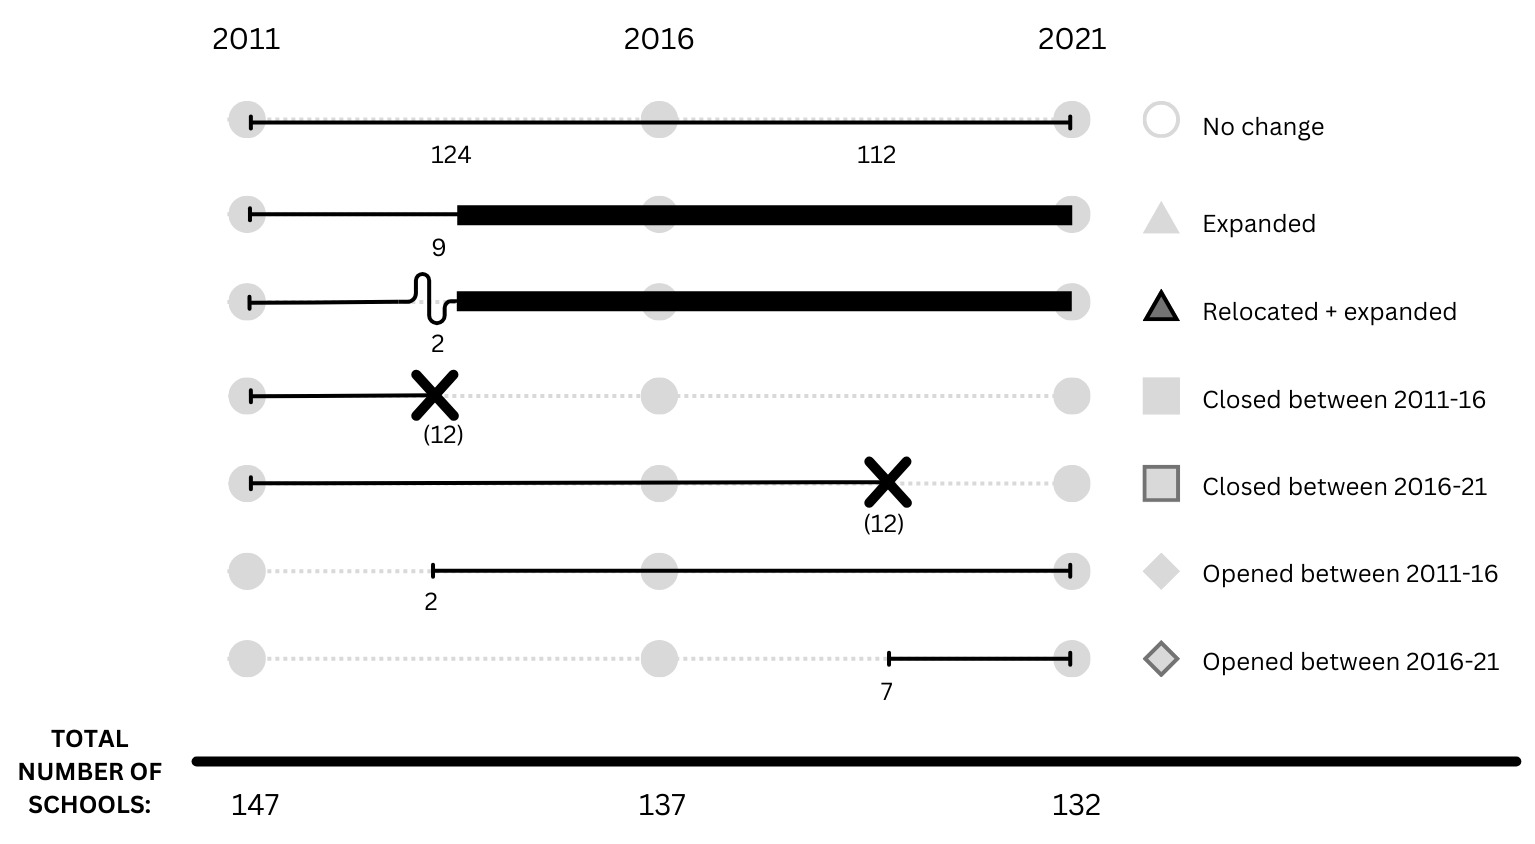
\includegraphics[width=1\textwidth,height=\textheight]{../Figures/Fig1.jpg}

}

\caption{\label{fig-Fig1}Overview of the number of schools in Hamilton
in 2011, 2016 and 2021 along with the type of school status change.}

\end{figure}%

For the spatial availability analysis, the capacity of each school is
also required for each year. This capacity is the number of `seats'
available at the school as calculated by the provincial Ministry of
Education. It is referred to as the on-the-ground capacity (OTGC) of a
school. However, it is important to note that schools rarely operate at
exactly their OTGC, they are typically either over-enrolled or
under-enrolled.

Current and historic OTGCs for schools are not publicly available
(Ontario 2017), so we used a set of known OTGC values gathered from
Pupil Accommodation Review documents and multivariate regression to
estimate and validate these values. Two regression models were created:
one for public schools and another for public catholic schools. The
independent variables in these models were 1) a dummy variable
indicating the level of the school (\emph{MidElem}, \emph{JrElem},
\emph{Elem}); 2) the school's building footprint (\emph{F}) in \(m^2\);
and 3) the school's Euclidean distance from the centroid of Hamilton's
central business district area (\emph{DistCBD}) in metres.

Formally, elementary schools are defined as schools that provide
instruction to any combination of grades between kindergarten to grade 8
(i.e.~typically children aged 5 to 14). As such, elementary includes
middle schools that only instruct grades 6 to 8 (\emph{MidElem}),
primary schools that only instruct kindergarten to grade 5 or 6
(\emph{JrElem}), and all grade elementary schools (\emph{Elem}) which
instruct all grades from kindergarten to grade 8. \emph{MidElem} and
\emph{JrElem} school grade instruction type is only present in the
public school board.

\begin{itemize}
\item
  The building footprint \emph{F} was retrieved from an archived spatial
  data set (Spatial 2015) and footprints from newer schools in 2016 and
  2021 from OSM (OpenStreetMap 2021).
\item
  \emph{DistCBD} was calculated `as the crow flies' from each school to
  the centroid of the Hamilton CBD (43.256684\(\circ\)N,
  79.869039\(\circ\)W). Notably, this variable can also be seen as a
  proxy for school construction age as older buildings in Hamilton are
  generally located closer to the CBD, the ``old'' Hamilton community
  (Merrall 2021).
\end{itemize}

Equations (\ref{eq:OTGC-public}) and (\ref{eq:OTGC-catholic}) are the
OTGC regression model for public schools and public catholic schools
respectively. As seen in Table \ref{Tab1-OTGC}, the coefficient of
determination for these models are quite high, at \(R^2 = 0.999\) and
\(R^2 = 0.998\) for the public and public catholic school boards
respectively, and the residual standard deviation is \(\sigma = 0.212\)
and \(sigma = 0.331\).

\begin{equation}
\label{eq:OTGC-public}
OTGC_{Public} = F^{0.346}-e^{0.00003*DistCBD}+e^{3.123*JrElem}+e^{3.752*Elem}+ e^{3.068*MidElem} 
\end{equation}

\begin{equation}
\label{eq:OTGC-catholic}
OTGC_{Public Catholic} =F^{0.471}-e^{0.00003*DistCBD}+e^{2.333*Elem}
\end{equation}


% Table created by stargazer v.5.2.3 by Marek Hlavac, Social Policy Institute. E-mail: marek.hlavac at gmail.com
% Date and time: Thu, Apr 25, 2024 - 1:03:02 PM
\begin{table}[!htbp] \centering 
  \caption{Estimated on-the-ground capacity (OTGC) (units of school seats available per school) regression results for public and public catholic school boards in Hamilton, Canada for years 2011 and 2016.} 
  \label{Tab1-OTGC} 
\begin{tabular}{@{\extracolsep{5pt}}lcc} 
\\[-1.8ex]\hline 
\hline \\[-1.8ex] 
 & \multicolumn{2}{c}{\textit{Dependent variable:}} \\ 
\\[-1.8ex] & \multicolumn{2}{c}{log(OTGC)} \\ 
\\[-1.8ex] & (Public) & (Public Catholic)\\ 
\hline \\[-1.8ex] 
 log(F) & 0.346$^{***}$ & 0.471$^{***}$ \\ 
  & (0.107) & (0.153) \\ 
  & & \\ 
 JrElem & 3.123$^{***}$ &  \\ 
  & (0.834) &  \\ 
  & & \\ 
 MidElem & 3.068$^{***}$ &  \\ 
  & (0.893) &  \\ 
  & & \\ 
 Elem & 3.752$^{***}$ &  2.333$^{*}$\\ 
  & (0.861) & (1.212) \\ 
  & & \\ 
 Sec & 4.094$^{***}$ &  2.936$^{**}$ \\ 
  & (0.978) & (1.398) \\ 
  & & \\ 
 urban.dist & $-$0.00003$^{***}$ & $-$0.00003$^{**}$ \\ 
  & (0.00001) & (0.00001) \\ 
  & & \\ 
\hline \\[-1.8ex] 
Observations & 42 & 42 \\ 
R$^{2}$ & 0.999 & 0.998 \\ 
Adjusted R$^{2}$ & 0.999 & 0.997 \\ 
Residual Std. Error & 0.212 (df = 36) & 0.331 (df = 38) \\ 
F Statistic & 6,189.428$^{***}$ (df = 6; 36) & 3,794.875$^{***}$ (df = 4; 38) \\ 
\hline 
\hline \\[-1.8ex] 
\textit{Note:}  & \multicolumn{2}{r}{$^{*}$p$<$0.1; $^{**}$p$<$0.05; $^{***}$p$<$0.01} \\ 
\end{tabular} 
\end{table} 


Taken together, Figure~\ref{fig-Fig2} displays the city's elementary
schools locations, status, and their observed or estimated OTGCs for
2011, 2016 and 2021. For additional context on the degree of residential
urbanization in Hamilton, the percentage of residential parcels
considered `urban' compared to `suburban' or `rural' is reflected at an
aggregated spatial unit across all six plots in Figure~\ref{fig-Fig2}.
This land-use classification is available within the 2021 residential
parcel file described in the following sub-section. In
Figure~\ref{fig-Fig2}, it can be seen that the majority of schools that
changed status are in the HWDSB, with OTGC decreasing in 2016 and 2021
compared to the previous year. Most school closures took place in the
central and eastern parts of Hamilton's urban area (Hamilton Central),
as well as in rural areas of western Hamilton (Flamborough). When
schools did open or expand, it was primarily in the more recently
urbanized southeastern area of Hamilton (Glanbrook), with a few also in
Hamilton Central to offset some of the lost capacity.

\begin{figure}

\centering{

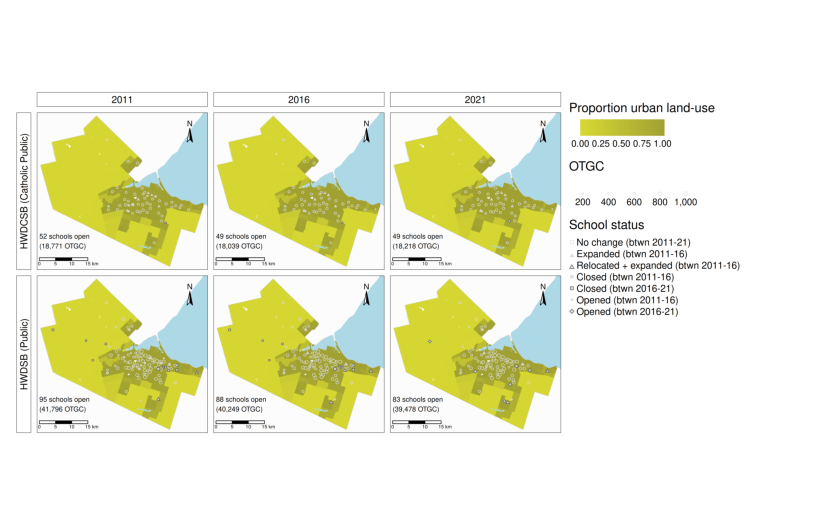
\includegraphics[width=1.2\textwidth,height=\textheight]{Manuscript_files/figure-pdf/fig-Fig2-1.pdf}

}

\caption{\label{fig-Fig2}The on-the-ground capacity (OTGC) of schools
and school status for year 2011, 2016 and 2021 for both the HWDSB and
HWCDSB. Schools are presented overtop a layer visualising the degree of
residential urbanisation in 2021.}

\end{figure}%

\subsection{Students, residential locations and low-income
prevelance}\label{students-residential-locations-and-low-income-prevelance}

Secondly, a detailed account of the average student population,
low-income prevalence of households, and where they may live is required
for each studied year.

Concerning the student population and poverty, information from the
2011, 2016 and 2021 Canadian Census (Canada 2011, 2016, 2021) was
sourced using the \{cancensus\} R package (Bergmann, Shkolnik, and
Jacobs 2021). The census releases population data by age group category,
so the population aged between 5-9 years and 10-14 years were retained.
A common poverty measure across all three census years is the low-income
after-tax measure (LIM-AT), which reflects the proportion of private
households that are below the median after-tax income in the region
(Government of Canada 2017). The LIM-AT prevalence for households with
children under 18 was retrained for this paper as there is no LIM-AT
prevalence tabulated for households with exclusively elementary-aged
children. Population and LIM-AT variables were taken at the
Dissemination Area (DA) level, the finest geographic unit publicly
available. DAs are designed by Statistics Canada with the aim of
population uniformity hence DAs greatly vary in area but represent
between approximately 400 and 700 (1st and 3rd quartile) in total
population. The population aged 5 to 14 and the proportion of LIM-AT are
visualised in the first and last rows in Figure~\ref{fig-Fig3}. LIM-AT
prevalence is notably more concentrated within the centre of Hamilton
(Hamilton Central) through 2011 to 2021, overlapping the most urbanised
land-use and the largest amount of schools closed
(Figure~\ref{fig-Fig2}). Also of note, LIM-AT prevalence drastically
decreased in 2021 as a result of Pandemic benefits that reduced income
inequality (Government of Canada 2022b).

Student residential locations were approximated at the level of
residential parcels. Centroids for parcels in 2011, 2016 and 2021 were
retrieved from Teranet (2009), representing \(134,340\), \(139,467\) and
\(143,890\) unique locations, respectively. Each residential unit in a
parcel was populated with the average number of children aged 5-14 in
the corresponding dissemination area (DA). Due to the proprietary nature
of the parcel data, the second row in Figure~\ref{fig-Fig3} shows an
aggregation of the information: the average rate of 5-14 year old
population per residential unit (parcel) at the DA level. Notably,
though the rate of 5-14 year old population per parcel is higher in more
peripheral (and rural) communities, there are many DAs within Hamilton
Central that have high rates and populations that are similar to those
in these more peripheral communities.

\begin{figure}[H]

\centering{

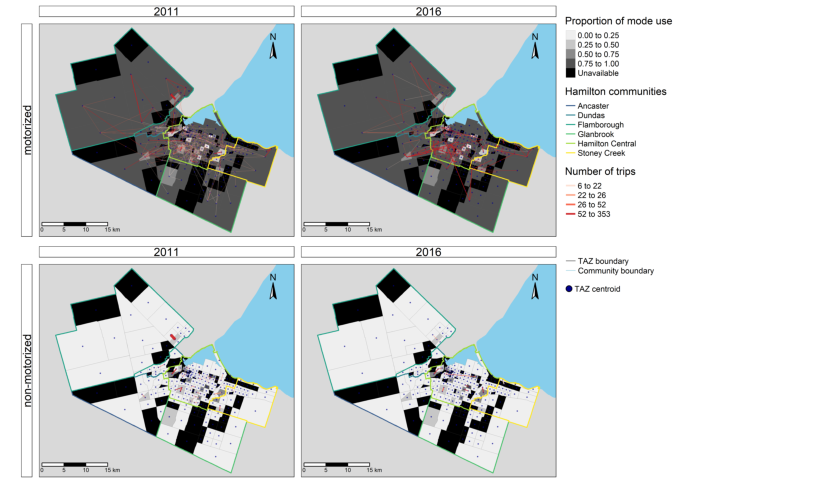
\includegraphics[width=1.2\textwidth,height=\textheight]{Manuscript_files/figure-pdf/fig-Fig3-1.pdf}

}

\caption{\label{fig-Fig3}The magnitude (top row) and rate per
residential unit (middle row) of elementary aged student population per
DA in 2011, 2016 and 2021. Bottom row: the proportion of low-income
households (prevelance of low-income after-tax, LIM-AT, measured by the
2011, 2016 and 2021 Canadian Census) with dependents under 18 years old
shown. All scales are represented in quartiles.}

\end{figure}%

\subsection{Trip length by mode}\label{trip-length-by-mode}

To reflect multimodal travel behaviour, two types of data was estimated
and compiled. The process for obtaining and preparing this data is
described as follows.

First, we retrieved information about the mode used and
origin-destination locations of home-to-school trips from the 2011 and
2016 TTS (Data Management Group 2018); the 2021 TTS survey is
unavailable at the time of writing so 2016 flows are assumed for the
2021 year. The TTS is a travel survey conducted in the Greater Golden
Horseshoe Area in Ontario typically every five years. With a target 5\%
sampling rate, the survey is expanded to be representative at the
traffic analysis zone (TAZ) level of geography. TAZ are spatial units
created for the purpose of the TTS and pulled from the R data package
\{TTS2016R\} (Soukhov and Páez 2023); a few DAs typically nest within
each TAZ. The trip-level travel data extracted for this paper represent
13,715 and 12,878 motorized trips (mode used includes private car
passenger, school bus, taxi, and transit) and 7,432 and 7,085
non-motorized trips (mode used includes walk and cycling) for 5 to 14
year olds from home-to-school in 2011 and 2016 respectively. The
intensity of modal home-to-school flows are visualised in
Figure~\ref{fig-Fig4} along with the boundaries of the TAZ and DAs. Also
in Figure~\ref{fig-Fig4}, not all TAZs capture an elementary school trip
by both modes. For this reason, the proportion of motorized modal share
is aggregated at the community level. Hamilton (Ancaster - 2011: 78\%and
2016:94\%, Dundas - 2011: 71\% and 2016: 67\%, Flamborough - 2011: 90\%
and 2016: 91\%, Glanbrook - 2011: 91\% and 2016: 78\%, Hamilton Central
- 2011: 55\% and 2016:50\%, and Stoney Creek - 2011: 71\% and 2016:
79\%).

\begin{figure}[H]

\centering{

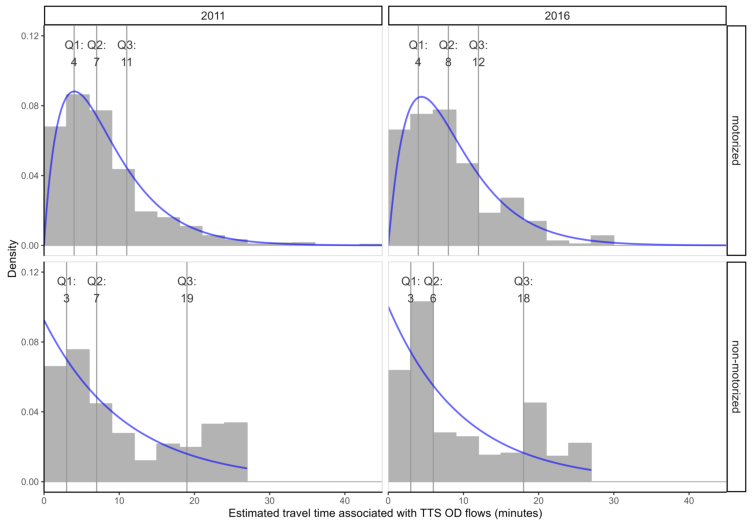
\includegraphics[width=1.2\textwidth,height=\textheight]{Manuscript_files/figure-pdf/fig-Fig4-1.pdf}

}

\caption{\label{fig-Fig4}The origin-destination flows from home-based
motorized and non-motorized school trips for students between 5-14 years
old as retrieved from TTS 2011 and 2016. Flows are mapped atop the
proportion of TAZ non/motorized modal share from the TTS 2011 and 2016,
DA boundaries, and Hamilton community boundaries.}

\end{figure}%

Next, travel times matrices for motorized and active travel were
calculated using \{r5r\} package (Pereira, Saraiva, et al. 2021). Travel
time matrices were estimated for all TAZ centroids to TAZ centroids
(matrices of size for 2011 and 2016: 234 x 234) as they are not reported
in the TTS. Additionally, matrices were estimated for all residential
parcels to schools (matrices of size 134,340 x 147 for 2011, 139,467 x
137 for 2016, and 143,890 x 132 for 2021) for additional granularity.
\{r5r\} is a R-based interface to the R5 routing engine (Conveyal
{[}2015{]} 2022). For simplicity, we assume motorized travel is by car
and non-motorized travel is by walking, as these are the most common
modes in their respective categories. For travel time calculations, we
set a maximum threshold of 60 minutes and use the free-flow
OpenStreetMap road network of Hamilton (Geofabrik 2022). While all car
trips are retained, walking trips over 27 minutes were filtered out.
This duration corresponds to a distance of 1.6 km (assuming a walking
speed of 3.6 km/h), which is the home-to-school distance threshold for
qualifying for motorized transport provided by the school board (HWDSB
2019). We use this threshold to assume that trips longer than 27 minutes
are highly unlikely to be made on foot.

In terms of the travel impedance function: we assume that children can
go to any elementary school, however, there is a preference for
facilities that are more proximate. Based on this assumption, we matched
the associated TAZ-to-TAZ travel times to all observed student-to-school
travel flows from the TTS; these are visualised as grey bar columns in
Figure~\ref{fig-Fig5}. Using these observed values, the
\emph{theoretical} trip length distribution (TLD) functions are
calibrated. TLDs can be interpreted as travel impedance functions as
they represent the propensity of realized travel, by trip length
(Horbachov and Svichynskyi 2018; Batista, Leclercq, and Geroliminis
2019). The TLDs are calibrated using the maximum likelihood and moment
matching techniques and the Nelder-Mead and Brent methods for direct
optimization available within the \{fitdistrplus\} R package
(Delignette-Muller and Dutang 2015). The theoretical TLD for each mode
and available study year is visualised in blue in Figure~\ref{fig-Fig5}.
Based on goodness-of-fit criteria and diagnostics, the gamma and
exponential distributions were selected for the motorized and
non-motorized modal distributions respectively. The gamma distribution
is defined by the shape (\(\alpha\)) parameter of 1.939 (2011) and 2.046
(2016) and the rate (\(\beta\)) of 0.233 (2011) and 0.236 (2016). The
exponential distribution is defined by the rate (\(\beta\)) parameter of
0.092 (2011) and 0.1 (2016). For reference, the gamma distribution and
the exponential distribution function are displayed in Equations
(\ref{eq:exp-dist}) and (\ref{eq:gamma-dist}) where \(x\) is \(c_{ij}\):

\begin{equation}
\label{eq:exp-dist}
f(x) = \beta e ^{-\beta x}
\end{equation}

\begin{equation}
\label{eq:gamma-dist}
\begin{aligned}
f(x, \alpha, \beta) = \frac {x^{\alpha-1}e^{-\frac{x}{\beta}}}{ \beta^{\alpha}\Gamma(\alpha)} \quad \text{for } 0 \leq x \leq \infty \\
\Gamma(\alpha) =  \int_{0}^{\infty} x^{\alpha-1}e^{-x} \,dx
\end{aligned}
\end{equation}

\begin{figure}[H]

\centering{

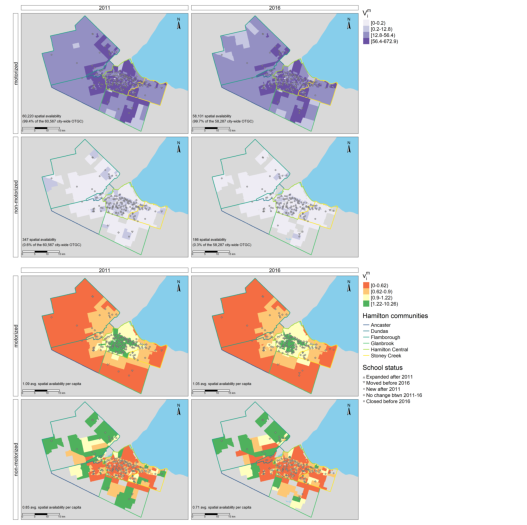
\includegraphics[width=1\textwidth,height=\textheight]{Manuscript_files/figure-pdf/fig-Fig5-1.pdf}

}

\caption{\label{fig-Fig5}Observed (grey bars) and theoretical (blue
curves) motorized and non-motorized impedance functions. Motorized
theoretical impedance function is based on the gamma distribution
function and non-motorized on the expoential distribution function}

\end{figure}%

Lastly, to achieve greater granularity, the TLDs calibrated using
TAZ-to-TAZ flows are used to estimate travel impedance values for each
parcel-to-school flow based on calculated parcel-to-school travel times.
These values represent the likelihood that students in a parcel will
travel to a school, informed by observed home-to-school flows from the
TTS.

\section{Methods: Multimodal spatial
availability}\label{methods-multimodal-spatial-availability}

Accessibility can be defined as the ``potential for spatial
interaction''. It is classically presented as the measure defined in
Hansen (1959) and takes the following general multimodal formulation:

\begin{equation}
\label{eq:multimodal-conventional-accessibility}
S_i^m = \sum_{j=1}^JO_j \cdot f^m(c_{ij}^m)
\end{equation}

\noindent where:

\begin{itemize}
\tightlist
\item
  \(m\) is a set of modes.
\item
  \(c_{ij}^m\) is a measure of the cost of moving between \(i\) and
  \(j\) for each \(m\).
\item
  \(f^m(\cdot)\) is an impedance function of \(c_{ij}^m\) for each
  \(m\); it can take the form of any monotonically decreasing function
  chosen based on positive or normative criteria (A. Páez, Scott, and
  Morency 2012).
\item
  \(i\) is a set of origin locations (\(i = 1,\cdots,N\)).
\item
  \(j\) is a set of destination locations (\(j = 1,\cdots,J\)).
\item
  \(O_j\) is the number of opportunities at location \(j\).
\item
  \(S\) is Hansen-type accessibility as weighted sum of opportunities.
\end{itemize}

As indicators of urban structure, Hansen-type accessibility measures
like Equation (\ref{eq:multimodal-conventional-accessibility}) are
informative in reflecting the magnitude of access but meaning of the
value itself is elusive. The significance of 10,000 accessible
school-seats is hard to pin down: how many opportunities must any single
student have access to? Furthermore, this opaque interpretation
especially is complicated when comparing accessibility of school seats
between years, such as different years as in this work. The
interpretability of Hansen-type accessibility has been discussed in
numerous studies, including recently by Hu and Downs (2019), Kelobonye
et al. (2020), and in greater depth by Merlin and Hu (2017) along with
Soukhov et al. (2023) and Soukhov et al. (2024). The interpretation of
accessibility depends on how many people demand the opportunity,
especially for exclusive opportunity-types like schools-seats (i.e., one
school-seat is for one student).

In this paper, our work benefits from new developments in accessibility
research, particularly the multimodal spatial availability measure
(Soukhov et al. 2023; Soukhov et al. 2024). Spatial availability is a
singly-constrained accessibility measure that can account for
competition of students using different modes potentially interacting
with scarce opportunities, such as school seats. The measure's sinlge
constraint ensures that the marginals at the destination are met and
thus the number of estimated school seats (opportunities) are preserved
and allocated proportionally to the mode-using student populations. This
proportional allocation of opportunities yields an interpretable and
meaningful measure of opportunity access, particularly when comparing
across modes, at the spatial resolution of a residential parcel, and
multiple time periods. See Soukhov et al. (2024) for further discussion.

The multimodal spatial availability \(V_{i}^m\) is defined as given by
Equation (\ref{eq:spatial-availability}):

\begin{equation}
\label{eq:spatial-availability}
V_{i}^{m} = \sum_{j=1}^J O_j\ F^{tm}_{ij}
\end{equation}

\noindent where:

\begin{itemize}
\tightlist
\item
  \(F^{tm}_{ij}\) is a balancing factor that depends on the population
  and cost of movement in the system as part of the gravity modelling
  framework and is captured in Equation (\ref{eq:balancing-factors}) for
  mode \(m\).
\item
  \(O_j\) is the number of opportunities at \(j\).
\item
  \(V_i^m\) is the number of spatially available opportunities from the
  perspective of \(i\) for mode \(m\).
\end{itemize}

\(F^{tm}_{ij}\) can also be understood as the joint probability of
allocating opportunities, where \(F^{pm}_{i}\) is the population-based
balancing factor that grants a larger share of opportunities to larger
\(m\) population spatial units and \(F^{cm}_{ij}\) is the
impedance-based balancing factor that grants a larger share of the
opportunities to less \(m\)-travel costly centers. Together
\(F^{tm}_{ij}\) ensures proportional allocation such that opportunities
\(O\) (like school-seats) are preserved for the whole region (i.e.,
\(O = \sum_{j} O_j = \sum_{i} V_i = \sum_{m}\sum_{i} V_i^m\) ) and is
reflected in Equation (\ref{eq:balancing-factors}):

\begin{equation}
\label{eq:balancing-factors}
F^{tm}_{ij} = \frac{F^{pm}_{i} \cdot F^{cm}_{ij}}{\sum_{i} F^{pm}_{i} \cdot F^{cm}_{ij}}
\end{equation}

\noindent where:

\begin{itemize}
\tightlist
\item
  The factor for allocation by population for each \(m\) at each \(i\)
  is \(F^{pm}_{i} = \frac{P_{i}^m}{\sum_{m}\sum_{i} P_{i}^m}\)
\item
  The factor for allocation by travel cost for each \(m\) at each \(i\)
  and \(j\) is
  \(F^{cm}_{ij} = \frac{f^m(c^m_{ij})}{\sum_{m}\sum_{i} f^m(c^m_{ij})}\)
\end{itemize}

It should be noted that, when summed over all spatial units in the
region, the population-based allocation factors \(F^{pm}_{i}\) always
equal 1 (\(\sum_{m}\sum_{i} F^{pm}_{i}= 1\)), likewise for
impedance-based allocation factors \(F^{cm}_{i}\)
(\(\sum_{m}\sum_{i} F^{cm}_{ij} = 1\)).

Hansen-type accessibility is not designed to preserve the number of
opportunities in the region, it simply counts the intensity of
opportunities that those in a zone can potentially interact with
(weighted by the friction of distance). Also, as discussed in Soukhov et
al. (2023), popular competitive accessibility measures such as the
two-step floating catchment area (2SFCA) (Joseph and Bantock 1982;
Weibull 1976; Shen 1998; Luo and Wang 2003) are internally inconsistent,
and the only way it preserves the number of opportunities is if the
effect of the impedance function is ignored when expanding the values of
opportunities per capita to obtain the total number of opportunities. On
the other hand, the proportional allocation procedure associated with
calculating multimodal spatial availability \(V_i^m\) consistently
returns a number of opportunities available to populations by mode that
matches the total number of opportunities in the region when summed. By
doing this consistently, it is possible to define a measure of
multimodal spatial availability per capita as presented in Equation
(\ref{eq:SA-per-capita}) for use as a benchmark to compare against the
regional opportunities per capita
(\(\frac{\sum_{j} O_j}{\sum_{i} P_i}\)).

\begin{equation}
\label{eq:SA-per-capita}
v_i^m = \frac{V_i^m}{P_i^m}
\end{equation}

To summarise the methodology and the data as described in Section 3,
multimodal spatial availability \(V_i^m\) and multimodal spatial
availability per student \(v_i^m\) is calculated for each parcel for
each studied year as follows:

\begin{itemize}
\tightlist
\item
  First, all residential parcels are associated to their respective
  census DA, TTS TAZ, and community boundary based on spatial location.
  Each parcel is assigned a number of `potential' motorized and
  non-motorized student aged population (from DA) and modal share (from
  TTS) to calculate a motorized and non-motorized population balancing
  factor \(F_{i}^{pm}\). For each parcel, the elementary-aged student
  population per parcel (Figure~\ref{fig-Fig3} second row) and the
  motorized and non-motorized share as informed by the TTS aggregated by
  community (Figure~\ref{fig-Fig4}) is retained.
\item
  Second, the school capacity \(O_j\) is estimated and associated with
  each school (Figure~\ref{fig-Fig2}). All residential locations are
  assumed to be able to access all schools by non-motorized and/or
  motorized mode. All origins (residential locations) can reach all
  schools by motorized mode, but few residential locations can reach
  schools within a 27 minute non-motorized trip.
\item
  Third, the motorized and non-motorized impedance-balancing factors
  \(F_{ij}^{cm}\) are calculated using a mode-specific impedance
  function (Figure~\ref{fig-Fig5}) based on the respective estimated
  travel times for each origin (parcel) to school combination. Using
  network estimated travel time sensitive to observed parcel origin to
  school destination flows conceptually addresses the aggregation error
  that could result from using less granular zonal units to represent
  origin/destinations (Kane and Kim 2020; Kwan 1998; Hewko,
  Smoyer-Tomic, and Hodgson 2002).
\item
  Finally, outputs from all three stages are joined together.
  \(F_{i}^{pm}\) joined with \(F_{ij}^{cm}\) yields the total balancing
  factor \(F^{tm}_{ij}\) which serves to proportionally allocate the
  school capacity \(O_j\) to each parcel. The value is multimodal
  spatial availability \(V_i^m\) which can be interpreted as the number
  of school-seats that are available to the mode-using population at
  that parcel. \(V_i^m\) is then summed and represented at the DA and
  community level along with the calculated \(v_i^m\) for
  interpretation.
\end{itemize}

\section{Results}\label{results}

To clarify terminology for readers, \(V_i^m\) is the number of
school-seats available to populations by mode (either motorized or
non-motorized) that matches the total number of opportunities in the
region as a result of the proportional allocation mechanism. In other
words, we describe \(V_i^m\) as the number of school-seats available to
a mode-using population. Each \(i\) (parcel, DA, or community) maintains
that singly-constrained relationship. \(v_i^m\) is the per capita
spatial availability to mode-using populations.

The probability density plots of the spatial availability values
\(V_i^m\) and the per capita spatial availability \(v_i^m\) values for
both modes (motorized and non-motorized) and all three years are
displayed in Figure~\ref{fig-Fig6} as a city-wide overview. The left
column displays parcel-level values, and the right reflects parcel-level
values aggregated at the 2021 DA grid. Both the parcel and DA level
values reflect the spatial unit at which they were calculated or
aggregated. However, the values of the \(V_i^m\) plots are not directly
comparable since the x- and y- axes are set at different scale limits to
highlight between year differences. However, overall trends in their
distribution can be compared: in all four \(V_i^m\) plots, the 2011 data
is more right-skewed than more current years, indicating that spatial
availability values used to be higher (e.g., more school-seat access).
School closures and consolidations had an impact despite the background
dynamics of assumed student population, mode use, travel time and parcel
location. The DA level \(V_i^m\) plots show the distribution of each DA
value, which is the summation of all parcel \(V_i^m\) values within a
DA. In 2011, DAs can be observed to also have more right-skewed spatial
availability values than previous years. In contrast, the 2016 and 2021
distributions are more intense and heavily skewed toward lower values.

Zonal per capita \(v_i^m\) values can be compared across the years as
the school-age population per spatial unit (e.g., parcel or DA) is used
to normalize the respective \(V_i^m\) value. \(v_i^m\) values are
presented in the bottom four plots of Figure~\ref{fig-Fig6}. It can be
observed that the same 2011 right-skewed trend persists across all
modes. Motorized mode-using students have access to more spatially
available school seats than non-motorized mode using students (in 2011,
approximately 1.3 school-seats per student as compared to 0.7 and in
2021 approximately 1.2 compared to 0.5). Due to school-seats per student
at the DA level being an interpretable aggregation, values at this level
will be the discussion focus of the remainder of this paper.

\begin{figure}[H]

\centering{

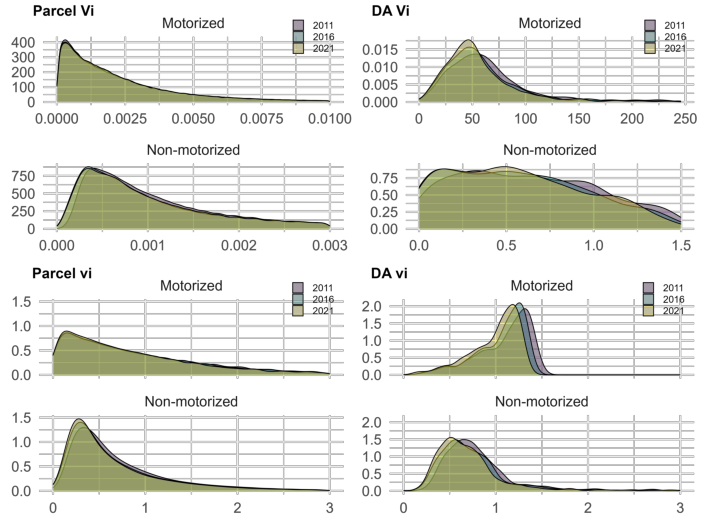
\includegraphics[width=1\textwidth,height=\textheight]{Manuscript_files/figure-pdf/fig-Fig6-1.pdf}

}

\caption{\label{fig-Fig6}Spatial availability (Vi) and per capita
spatial availability (vi) probability density distributions for the city
of Hamilton in 2011, 2016 and 2021. Aggregated at the parcel level (left
column) and DA level (right column).}

\end{figure}%

Representing the right column of Figure~\ref{fig-Fig6} spatially,
Figure~\ref{fig-Fig7} displays the spatial availability for each DA for
a given mode-using population \(m\) (e.g., the sum of school seat
availability per parcel in each DA for motorized or non-motorized
students). Figure~\ref{fig-Fig7} visualizes the spatial distribution of
motorized and non-motorized school seat availability for 2011, 2016, and
2021. As a reminder, the sum of \(V_i^m\) values for both motorized and
non-motorized populations in a given year equals the city-wide OTGC
(i.e., school seats across both the HWDSB and HWCDSB). This is due to
\(V_i^m\)'s proportional allocation mechanism, singly-constraining
opportunities through the proportion allocation balancing factors. In
this way, \(V_i^m\) values can be interpreted as a proportion of the
total OTGC for that year, as the sum of \(V_i^m\) for both modes in a
year equals the total OTGC for that year.

Referring to the first two rows of \(V_i^m\) plots in
Figure~\ref{fig-Fig7} (purples), it is notable that the magnitudes of
\(V_i^m\) values for the motorized and non-motorized populations are
tremendously different. Again, each \(V_i^m\) value reflects the number
of school seats spatially available to the mode-using population at that
zonal level, so due to the lower non-motorized modal share (refer to
Figure~\ref{fig-Fig4}), non-motorized values will be lower. However,
both mode-using populations have higher spatial availability values
(darker purples) in DAs that are more proximate to schools. Hence, all
DAs have higher values within Hamilton Central and those more proximate
to schools in less-urban communities. This trend persists across 2011,
2016 and 2021, aligning with intuition: populations with shorter travel
times to with relatively greater schools are calculated to have high
school seat spatial availability. Motorized populations have shorter
travel times at DAs further in distance from schools, while
non-motorized populations are only competitive at proximate distances.

The bottom two rows of \(v_i^m\) plots in Figure~\ref{fig-Fig7} (yellows
to greens) demonstrate the spatial availability per mode-using student
population e.g., \(V_i^m\) divided by the number of students aged 5-14
using a motorized mode or non-motorized mode. It is notable that for
motorized populations, their spatial availability per student is above 1
(green) within the center of the city. Conversely, this rate is only
available to non-motorized populations in DAs that are in less-densely
populated rural areas that are school proximate and very few pockets of
Hamilton Central in 2011 and 2016. In 2021, even fewer DAs within
Hamilton Central have non-motorized spatial availability rates above 1.

\begin{figure}[H]

\centering{

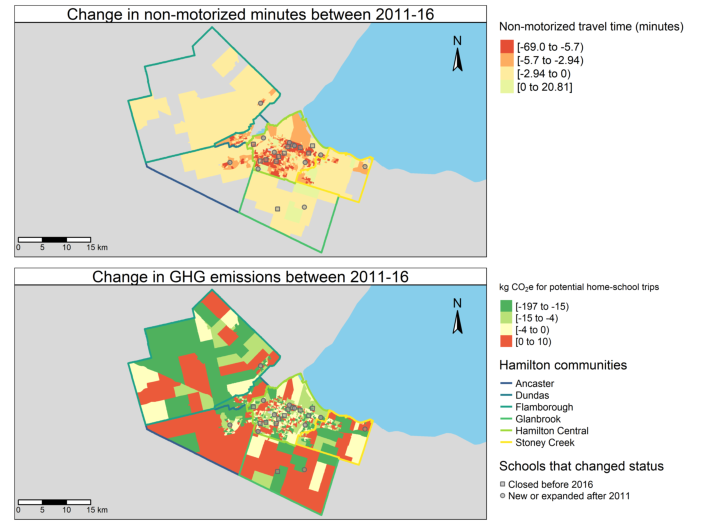
\includegraphics[width=1.2\textwidth,height=\textheight]{Manuscript_files/figure-pdf/fig-Fig7-1.pdf}

}

\caption{\label{fig-Fig7}Multimodal spatial availability (purples) and
spatial availability per mode-using student (diverging reds and greens)
aggregated at the DA level for 2011, 2016 and 2021. Scales are
represented in deciles.}

\end{figure}%

To further explore these changes, the difference in \(V_i^m\) (first two
rows) and difference in \(v_i^m\) (second two rows) between 2011-2016,
2016-2021 and overall between 2011-2021 are displayed in
Figure~\ref{fig-Fig8} along with schools that changed during that time
period. 2011-2016 and 2016-2021 add together to equal 2011-2021 changes
quite clearly, e.g.~in the third row, the 2011-16 plots a small decrease
within the core of the city, and 2016-2021 demonstrates a more
significant decrease in the core and western peripheral communities.
Together, 2011-2021 plot reflects the changes in these two plots.

A few notable spatial trends can be observed in Figure~\ref{fig-Fig8}.
First, DAs in proximity to schools that closed (square points) see
losses in \(V_i^m\) (reds) for both motorized and especially
non-motorized populations. For non-motorized populations, all closed
school resulted in a decrease in \(V_i^m\). The majority of school
closures took place in the central and eastern parts of Hamilton's urban
area (Hamilton Central), as well as in rural areas of western Hamilton
(Flamborough). Hence, losses characterise those neighbourhoods.
Secondly, gains in \(V_i^m\) (blues) are seen where schools are opened
(diamond points) or expanded (triangle points), especially for motorized
populations. These gains are most notably in the more recently urbanized
southeastern area of Hamilton (Glanbrook), along with a few pockets of
DAs in proximity to new or expanded schools in Hamilton Central.
Thirdly, the concentration of students in proximity to schools and the
extent of their OTGC matters from the perspecitve of modal advantage. In
areas with fewer proximate school options and lower OTGC relative to the
amount of students, a change in a school results in a big impact on
spatial availability values. For instance, in the community of Ancaster,
one school expanded in the rural area in this community between
2011-2016. The motorized student population, especially in rural DAs,
saw gains in spatial availability while non-motorized populations saw
losses. Students in proximity to the schools in Ancaster have high
non-motorized spatial availability, but when the school was expanded
(and due to an under-served population) motorized populations saw an
increase in spatial availability at the direct expense of non-motorized
populations' spatial availability.

Exploring changes in \(V_i^m\) provides a holistic view of spatial
availability for a given DA. However, if the focus is on the ratio of
spatial availability per student, the bottom two rows in
Figure~\ref{fig-Fig8} offer more insight. For instance, a community may
have had an initially average rate of school seats per student but is
expecting an increase in student population so it expands a school.
However, due to an increase in population, the spatial availability per
student overall still decreases between these two time periods. This
case appears to occur in Ancaster between 2011 to 2016: while motorized
\(V_i^m\) increased, motorized \(v_i^m\) slightly decreased, and
non-motorized \(v_i^m\) decreased relatively more than non-motorized
\(V_i^m\). As shown in Figure~\ref{fig-Fig3}, the student population and
the number of students per residential unit increased more rapidly than
the expanded school could accommodate, leading to a decrease in
\(v_i^m\) values in DAs proximate to expanded schools.

Similarly, in the southeastern community of Glanbrook, student
populations grew from 2011 to 2021, and new schools opened. However,
\(v_i^m\) rates decreased because OTGC did not keep pace with student
population growth. As another example, in Hamilton Central and the
eastern community of Stoney Creek, changes in \(V_i^m\) are unpatterned,
while \(v_i^m\) demonstrate more uniform decreases, with the pattern
varying by modal-range for motorized versus non-motorized populations.
In these communities, the student population remained relatively stable,
though OTGC decreased overall. \(v_i^m\) is illuminating to consider
when comparing changes in spatial availability rates.

\begin{figure}[H]

\centering{

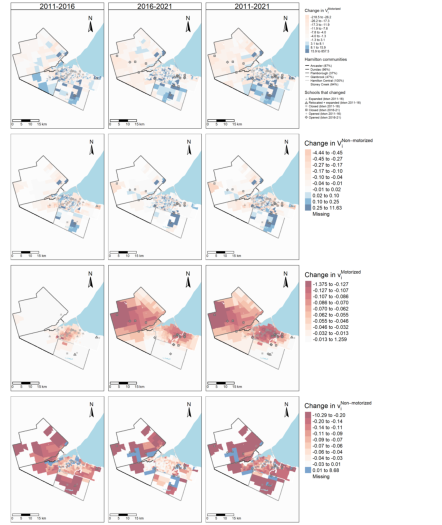
\includegraphics[width=1.2\textwidth,height=\textheight]{Manuscript_files/figure-pdf/fig-Fig8-1.pdf}

}

\caption{\label{fig-Fig8}Change in multimodal spatial availability and
spatial availability per mode-using student from 2011 to 2016, 2016 to
2021, and together from 2011 to 2021. Change is the subtraction of
parcel-level results in that given year and summed for each DA in the
2021 Canadian Census DA grid. Scales are represented in deciles.}

\end{figure}%

Changes in multimodal spatial availability is important: A summary of
spatial availability per Hamilton community and associated dimensions in
2021, along with the percentage change between 2011 and 2021, is
presented in Table~\ref{tbl-Tab2}.

\global\setlength{\Oldarrayrulewidth}{\arrayrulewidth}

\global\setlength{\Oldtabcolsep}{\tabcolsep}

\setlength{\tabcolsep}{2pt}

\renewcommand*{\arraystretch}{1.5}



\providecommand{\ascline}[3]{\noalign{\global\arrayrulewidth #1}\arrayrulecolor[HTML]{#2}\cline{#3}}

\begin{longtable}[c]{ccccccccccccc}

\caption{\label{tbl-Tab2}Spatial availability and associated dimensions
aggregated by communities in 2011 and percentage change by 2021.
Motorized and non-motorized values are labeled with mt and nmt
respectively.}

\tabularnewline

\hhline{>{\arrayrulecolor[HTML]{666666}\global\arrayrulewidth=1.5pt}->{\arrayrulecolor[HTML]{666666}\global\arrayrulewidth=1.5pt}->{\arrayrulecolor[HTML]{666666}\global\arrayrulewidth=1.5pt}->{\arrayrulecolor[HTML]{666666}\global\arrayrulewidth=1.5pt}->{\arrayrulecolor[HTML]{666666}\global\arrayrulewidth=1.5pt}->{\arrayrulecolor[HTML]{666666}\global\arrayrulewidth=1.5pt}->{\arrayrulecolor[HTML]{666666}\global\arrayrulewidth=1.5pt}->{\arrayrulecolor[HTML]{666666}\global\arrayrulewidth=1.5pt}->{\arrayrulecolor[HTML]{666666}\global\arrayrulewidth=1.5pt}->{\arrayrulecolor[HTML]{666666}\global\arrayrulewidth=1.5pt}->{\arrayrulecolor[HTML]{666666}\global\arrayrulewidth=1.5pt}->{\arrayrulecolor[HTML]{666666}\global\arrayrulewidth=1.5pt}->{\arrayrulecolor[HTML]{666666}\global\arrayrulewidth=1.5pt}-}

\multicolumn{1}{>{}c}{\textcolor[HTML]{000000}{\fontsize{7}{7}\selectfont{\global\setmainfont{Arial}{\textbf{}}}}} & \multicolumn{1}{>{}c}{\textcolor[HTML]{000000}{\fontsize{7}{7}\selectfont{\global\setmainfont{Arial}{\textbf{Hamilton\ C.}}}}} & \multicolumn{1}{>{}c}{\textcolor[HTML]{000000}{\fontsize{7}{7}\selectfont{\global\setmainfont{Arial}{\textbf{\%\ Δ}}}}} & \multicolumn{1}{>{}c}{\textcolor[HTML]{000000}{\fontsize{7}{7}\selectfont{\global\setmainfont{Arial}{\textbf{Dundas}}}}} & \multicolumn{1}{>{}c}{\textcolor[HTML]{000000}{\fontsize{7}{7}\selectfont{\global\setmainfont{Arial}{\textbf{\%\ Δ}}}}} & \multicolumn{1}{>{}c}{\textcolor[HTML]{000000}{\fontsize{7}{7}\selectfont{\global\setmainfont{Arial}{\textbf{Stoney\ Creek}}}}} & \multicolumn{1}{>{}c}{\textcolor[HTML]{000000}{\fontsize{7}{7}\selectfont{\global\setmainfont{Arial}{\textbf{\%\ Δ}}}}} & \multicolumn{1}{>{}c}{\textcolor[HTML]{000000}{\fontsize{7}{7}\selectfont{\global\setmainfont{Arial}{\textbf{Glanbrook}}}}} & \multicolumn{1}{>{}c}{\textcolor[HTML]{000000}{\fontsize{7}{7}\selectfont{\global\setmainfont{Arial}{\textbf{\%\ Δ}}}}} & \multicolumn{1}{>{}c}{\textcolor[HTML]{000000}{\fontsize{7}{7}\selectfont{\global\setmainfont{Arial}{\textbf{Flamborough}}}}} & \multicolumn{1}{>{}c}{\textcolor[HTML]{000000}{\fontsize{7}{7}\selectfont{\global\setmainfont{Arial}{\textbf{\%\ Δ}}}}} & \multicolumn{1}{>{}c}{\textcolor[HTML]{000000}{\fontsize{7}{7}\selectfont{\global\setmainfont{Arial}{\textbf{Ancaster}}}}} & \multicolumn{1}{>{}c}{\textcolor[HTML]{000000}{\fontsize{7}{7}\selectfont{\global\setmainfont{Arial}{\textbf{\%\ Δ}}}}} \\

\noalign{\global\arrayrulewidth 0pt}\arrayrulecolor[HTML]{000000}

\hhline{>{\arrayrulecolor[HTML]{666666}\global\arrayrulewidth=1.5pt}->{\arrayrulecolor[HTML]{666666}\global\arrayrulewidth=1.5pt}->{\arrayrulecolor[HTML]{666666}\global\arrayrulewidth=1.5pt}->{\arrayrulecolor[HTML]{666666}\global\arrayrulewidth=1.5pt}->{\arrayrulecolor[HTML]{666666}\global\arrayrulewidth=1.5pt}->{\arrayrulecolor[HTML]{666666}\global\arrayrulewidth=1.5pt}->{\arrayrulecolor[HTML]{666666}\global\arrayrulewidth=1.5pt}->{\arrayrulecolor[HTML]{666666}\global\arrayrulewidth=1.5pt}->{\arrayrulecolor[HTML]{666666}\global\arrayrulewidth=1.5pt}->{\arrayrulecolor[HTML]{666666}\global\arrayrulewidth=1.5pt}->{\arrayrulecolor[HTML]{666666}\global\arrayrulewidth=1.5pt}->{\arrayrulecolor[HTML]{666666}\global\arrayrulewidth=1.5pt}->{\arrayrulecolor[HTML]{666666}\global\arrayrulewidth=1.5pt}-}\endfirsthead 

\hhline{>{\arrayrulecolor[HTML]{666666}\global\arrayrulewidth=1.5pt}->{\arrayrulecolor[HTML]{666666}\global\arrayrulewidth=1.5pt}->{\arrayrulecolor[HTML]{666666}\global\arrayrulewidth=1.5pt}->{\arrayrulecolor[HTML]{666666}\global\arrayrulewidth=1.5pt}->{\arrayrulecolor[HTML]{666666}\global\arrayrulewidth=1.5pt}->{\arrayrulecolor[HTML]{666666}\global\arrayrulewidth=1.5pt}->{\arrayrulecolor[HTML]{666666}\global\arrayrulewidth=1.5pt}->{\arrayrulecolor[HTML]{666666}\global\arrayrulewidth=1.5pt}->{\arrayrulecolor[HTML]{666666}\global\arrayrulewidth=1.5pt}->{\arrayrulecolor[HTML]{666666}\global\arrayrulewidth=1.5pt}->{\arrayrulecolor[HTML]{666666}\global\arrayrulewidth=1.5pt}->{\arrayrulecolor[HTML]{666666}\global\arrayrulewidth=1.5pt}->{\arrayrulecolor[HTML]{666666}\global\arrayrulewidth=1.5pt}-}

\multicolumn{1}{>{}c}{\textcolor[HTML]{000000}{\fontsize{7}{7}\selectfont{\global\setmainfont{Arial}{\textbf{}}}}} & \multicolumn{1}{>{}c}{\textcolor[HTML]{000000}{\fontsize{7}{7}\selectfont{\global\setmainfont{Arial}{\textbf{Hamilton\ C.}}}}} & \multicolumn{1}{>{}c}{\textcolor[HTML]{000000}{\fontsize{7}{7}\selectfont{\global\setmainfont{Arial}{\textbf{\%\ Δ}}}}} & \multicolumn{1}{>{}c}{\textcolor[HTML]{000000}{\fontsize{7}{7}\selectfont{\global\setmainfont{Arial}{\textbf{Dundas}}}}} & \multicolumn{1}{>{}c}{\textcolor[HTML]{000000}{\fontsize{7}{7}\selectfont{\global\setmainfont{Arial}{\textbf{\%\ Δ}}}}} & \multicolumn{1}{>{}c}{\textcolor[HTML]{000000}{\fontsize{7}{7}\selectfont{\global\setmainfont{Arial}{\textbf{Stoney\ Creek}}}}} & \multicolumn{1}{>{}c}{\textcolor[HTML]{000000}{\fontsize{7}{7}\selectfont{\global\setmainfont{Arial}{\textbf{\%\ Δ}}}}} & \multicolumn{1}{>{}c}{\textcolor[HTML]{000000}{\fontsize{7}{7}\selectfont{\global\setmainfont{Arial}{\textbf{Glanbrook}}}}} & \multicolumn{1}{>{}c}{\textcolor[HTML]{000000}{\fontsize{7}{7}\selectfont{\global\setmainfont{Arial}{\textbf{\%\ Δ}}}}} & \multicolumn{1}{>{}c}{\textcolor[HTML]{000000}{\fontsize{7}{7}\selectfont{\global\setmainfont{Arial}{\textbf{Flamborough}}}}} & \multicolumn{1}{>{}c}{\textcolor[HTML]{000000}{\fontsize{7}{7}\selectfont{\global\setmainfont{Arial}{\textbf{\%\ Δ}}}}} & \multicolumn{1}{>{}c}{\textcolor[HTML]{000000}{\fontsize{7}{7}\selectfont{\global\setmainfont{Arial}{\textbf{Ancaster}}}}} & \multicolumn{1}{>{}c}{\textcolor[HTML]{000000}{\fontsize{7}{7}\selectfont{\global\setmainfont{Arial}{\textbf{\%\ Δ}}}}} \\

\noalign{\global\arrayrulewidth 0pt}\arrayrulecolor[HTML]{000000}

\hhline{>{\arrayrulecolor[HTML]{666666}\global\arrayrulewidth=1.5pt}->{\arrayrulecolor[HTML]{666666}\global\arrayrulewidth=1.5pt}->{\arrayrulecolor[HTML]{666666}\global\arrayrulewidth=1.5pt}->{\arrayrulecolor[HTML]{666666}\global\arrayrulewidth=1.5pt}->{\arrayrulecolor[HTML]{666666}\global\arrayrulewidth=1.5pt}->{\arrayrulecolor[HTML]{666666}\global\arrayrulewidth=1.5pt}->{\arrayrulecolor[HTML]{666666}\global\arrayrulewidth=1.5pt}->{\arrayrulecolor[HTML]{666666}\global\arrayrulewidth=1.5pt}->{\arrayrulecolor[HTML]{666666}\global\arrayrulewidth=1.5pt}->{\arrayrulecolor[HTML]{666666}\global\arrayrulewidth=1.5pt}->{\arrayrulecolor[HTML]{666666}\global\arrayrulewidth=1.5pt}->{\arrayrulecolor[HTML]{666666}\global\arrayrulewidth=1.5pt}->{\arrayrulecolor[HTML]{666666}\global\arrayrulewidth=1.5pt}-}\endhead



\multicolumn{1}{>{}c}{\textcolor[HTML]{000000}{\fontsize{7}{7}\selectfont{\global\setmainfont{Arial}{LIM-AT}}}} & \multicolumn{1}{>{}c}{\textcolor[HTML]{000000}{\fontsize{7}{7}\selectfont{\global\setmainfont{Arial}{23.9}}}} & \multicolumn{1}{>{\cellcolor[HTML]{F4FBF3}}c}{\textcolor[HTML]{000000}{\fontsize{7}{7}\selectfont{\global\setmainfont{Arial}{13.2\%}}}} & \multicolumn{1}{>{}c}{\textcolor[HTML]{000000}{\fontsize{7}{7}\selectfont{\global\setmainfont{Arial}{11.3}}}} & \multicolumn{1}{>{\cellcolor[HTML]{F6FCF5}}c}{\textcolor[HTML]{000000}{\fontsize{7}{7}\selectfont{\global\setmainfont{Arial}{10.6\%}}}} & \multicolumn{1}{>{}c}{\textcolor[HTML]{000000}{\fontsize{7}{7}\selectfont{\global\setmainfont{Arial}{10.8}}}} & \multicolumn{1}{>{\cellcolor[HTML]{F7FCF7}}c}{\textcolor[HTML]{000000}{\fontsize{7}{7}\selectfont{\global\setmainfont{Arial}{9.1\%}}}} & \multicolumn{1}{>{}c}{\textcolor[HTML]{000000}{\fontsize{7}{7}\selectfont{\global\setmainfont{Arial}{8.3}}}} & \multicolumn{1}{>{\cellcolor[HTML]{FFFAF8}}c}{\textcolor[HTML]{000000}{\fontsize{7}{7}\selectfont{\global\setmainfont{Arial}{-2.5\%}}}} & \multicolumn{1}{>{}c}{\textcolor[HTML]{000000}{\fontsize{7}{7}\selectfont{\global\setmainfont{Arial}{7.2}}}} & \multicolumn{1}{>{\cellcolor[HTML]{FAFDFA}}c}{\textcolor[HTML]{000000}{\fontsize{7}{7}\selectfont{\global\setmainfont{Arial}{5.4\%}}}} & \multicolumn{1}{>{}c}{\textcolor[HTML]{000000}{\fontsize{7}{7}\selectfont{\global\setmainfont{Arial}{7.1}}}} & \multicolumn{1}{>{\cellcolor[HTML]{EAF7E9}}c}{\textcolor[HTML]{000000}{\fontsize{7}{7}\selectfont{\global\setmainfont{Arial}{24.9\%}}}} \\

\noalign{\global\arrayrulewidth 0pt}\arrayrulecolor[HTML]{000000}





\multicolumn{1}{>{}c}{\textcolor[HTML]{000000}{\fontsize{7}{7}\selectfont{\global\setmainfont{Arial}{Kid\ pop.}}}} & \multicolumn{1}{>{}c}{\textcolor[HTML]{000000}{\fontsize{7}{7}\selectfont{\global\setmainfont{Arial}{35,310.6}}}} & \multicolumn{1}{>{\cellcolor[HTML]{FFF9F7}}c}{\textcolor[HTML]{000000}{\fontsize{7}{7}\selectfont{\global\setmainfont{Arial}{-3.2\%}}}} & \multicolumn{1}{>{}c}{\textcolor[HTML]{000000}{\fontsize{7}{7}\selectfont{\global\setmainfont{Arial}{2,590.0}}}} & \multicolumn{1}{>{\cellcolor[HTML]{FFE3D9}}c}{\textcolor[HTML]{000000}{\fontsize{7}{7}\selectfont{\global\setmainfont{Arial}{-14.7\%}}}} & \multicolumn{1}{>{}c}{\textcolor[HTML]{000000}{\fontsize{7}{7}\selectfont{\global\setmainfont{Arial}{7,514.8}}}} & \multicolumn{1}{>{\cellcolor[HTML]{EEF9ED}}c}{\textcolor[HTML]{000000}{\fontsize{7}{7}\selectfont{\global\setmainfont{Arial}{20.0\%}}}} & \multicolumn{1}{>{}c}{\textcolor[HTML]{000000}{\fontsize{7}{7}\selectfont{\global\setmainfont{Arial}{2,639.7}}}} & \multicolumn{1}{>{\cellcolor[HTML]{A2DB9F}}c}{\textcolor[HTML]{000000}{\fontsize{7}{7}\selectfont{\global\setmainfont{Arial}{108.9\%}}}} & \multicolumn{1}{>{}c}{\textcolor[HTML]{000000}{\fontsize{7}{7}\selectfont{\global\setmainfont{Arial}{5,365.0}}}} & \multicolumn{1}{>{\cellcolor[HTML]{F8FCF7}}c}{\textcolor[HTML]{000000}{\fontsize{7}{7}\selectfont{\global\setmainfont{Arial}{8.7\%}}}} & \multicolumn{1}{>{}c}{\textcolor[HTML]{000000}{\fontsize{7}{7}\selectfont{\global\setmainfont{Arial}{4,845.0}}}} & \multicolumn{1}{>{\cellcolor[HTML]{F5FBF4}}c}{\textcolor[HTML]{000000}{\fontsize{7}{7}\selectfont{\global\setmainfont{Arial}{12.4\%}}}} \\

\noalign{\global\arrayrulewidth 0pt}\arrayrulecolor[HTML]{000000}





\multicolumn{1}{>{}c}{\textcolor[HTML]{000000}{\fontsize{7}{7}\selectfont{\global\setmainfont{Arial}{OTGC}}}} & \multicolumn{1}{>{}c}{\textcolor[HTML]{000000}{\fontsize{7}{7}\selectfont{\global\setmainfont{Arial}{39,889.1}}}} & \multicolumn{1}{>{\cellcolor[HTML]{FFECE5}}c}{\textcolor[HTML]{000000}{\fontsize{7}{7}\selectfont{\global\setmainfont{Arial}{-9.8\%}}}} & \multicolumn{1}{>{}c}{\textcolor[HTML]{000000}{\fontsize{7}{7}\selectfont{\global\setmainfont{Arial}{2,377.0}}}} & \multicolumn{1}{>{\cellcolor[HTML]{FFFFFF}}c}{\textcolor[HTML]{000000}{\fontsize{7}{7}\selectfont{\global\setmainfont{Arial}{0.0\%}}}} & \multicolumn{1}{>{}c}{\textcolor[HTML]{000000}{\fontsize{7}{7}\selectfont{\global\setmainfont{Arial}{9,010.2}}}} & \multicolumn{1}{>{\cellcolor[HTML]{FFF1EB}}c}{\textcolor[HTML]{000000}{\fontsize{7}{7}\selectfont{\global\setmainfont{Arial}{-7.6\%}}}} & \multicolumn{1}{>{}c}{\textcolor[HTML]{000000}{\fontsize{7}{7}\selectfont{\global\setmainfont{Arial}{1,313.5}}}} & \multicolumn{1}{>{\cellcolor[HTML]{91D58F}}c}{\textcolor[HTML]{000000}{\fontsize{7}{7}\selectfont{\global\setmainfont{Arial}{127.6\%}}}} & \multicolumn{1}{>{}c}{\textcolor[HTML]{000000}{\fontsize{7}{7}\selectfont{\global\setmainfont{Arial}{4,590.7}}}} & \multicolumn{1}{>{\cellcolor[HTML]{FFF1EB}}c}{\textcolor[HTML]{000000}{\fontsize{7}{7}\selectfont{\global\setmainfont{Arial}{-7.5\%}}}} & \multicolumn{1}{>{}c}{\textcolor[HTML]{000000}{\fontsize{7}{7}\selectfont{\global\setmainfont{Arial}{3,386.9}}}} & \multicolumn{1}{>{\cellcolor[HTML]{F6FBF5}}c}{\textcolor[HTML]{000000}{\fontsize{7}{7}\selectfont{\global\setmainfont{Arial}{11.1\%}}}} \\

\noalign{\global\arrayrulewidth 0pt}\arrayrulecolor[HTML]{000000}

\hhline{>{\arrayrulecolor[HTML]{666666}\global\arrayrulewidth=1pt}->{\arrayrulecolor[HTML]{666666}\global\arrayrulewidth=1pt}->{\arrayrulecolor[HTML]{666666}\global\arrayrulewidth=1pt}->{\arrayrulecolor[HTML]{666666}\global\arrayrulewidth=1pt}->{\arrayrulecolor[HTML]{666666}\global\arrayrulewidth=1pt}->{\arrayrulecolor[HTML]{666666}\global\arrayrulewidth=1pt}->{\arrayrulecolor[HTML]{666666}\global\arrayrulewidth=1pt}->{\arrayrulecolor[HTML]{666666}\global\arrayrulewidth=1pt}->{\arrayrulecolor[HTML]{666666}\global\arrayrulewidth=1pt}->{\arrayrulecolor[HTML]{666666}\global\arrayrulewidth=1pt}->{\arrayrulecolor[HTML]{666666}\global\arrayrulewidth=1pt}->{\arrayrulecolor[HTML]{666666}\global\arrayrulewidth=1pt}->{\arrayrulecolor[HTML]{666666}\global\arrayrulewidth=1pt}-}



\multicolumn{13}{>{}c}{\textcolor[HTML]{000000}{\fontsize{7}{7}\selectfont{\global\setmainfont{Arial}{\textbf{Motorized}}}}} \\

\noalign{\global\arrayrulewidth 0pt}\arrayrulecolor[HTML]{000000}

\hhline{>{\arrayrulecolor[HTML]{666666}\global\arrayrulewidth=1pt}->{\arrayrulecolor[HTML]{666666}\global\arrayrulewidth=1pt}->{\arrayrulecolor[HTML]{666666}\global\arrayrulewidth=1pt}->{\arrayrulecolor[HTML]{666666}\global\arrayrulewidth=1pt}->{\arrayrulecolor[HTML]{666666}\global\arrayrulewidth=1pt}->{\arrayrulecolor[HTML]{666666}\global\arrayrulewidth=1pt}->{\arrayrulecolor[HTML]{666666}\global\arrayrulewidth=1pt}->{\arrayrulecolor[HTML]{666666}\global\arrayrulewidth=1pt}->{\arrayrulecolor[HTML]{666666}\global\arrayrulewidth=1pt}->{\arrayrulecolor[HTML]{666666}\global\arrayrulewidth=1pt}->{\arrayrulecolor[HTML]{666666}\global\arrayrulewidth=1pt}->{\arrayrulecolor[HTML]{666666}\global\arrayrulewidth=1pt}->{\arrayrulecolor[HTML]{666666}\global\arrayrulewidth=1pt}-}



\multicolumn{1}{>{}c}{\textcolor[HTML]{000000}{\fontsize{7}{7}\selectfont{\global\setmainfont{Arial}{V\ (mt)}}}} & \multicolumn{1}{>{}c}{\textcolor[HTML]{000000}{\fontsize{7}{7}\selectfont{\global\setmainfont{Arial}{42,527.8}}}} & \multicolumn{1}{>{\cellcolor[HTML]{FFE9E1}}c}{\textcolor[HTML]{000000}{\fontsize{7}{7}\selectfont{\global\setmainfont{Arial}{-11.6\%}}}} & \multicolumn{1}{>{}c}{\textcolor[HTML]{000000}{\fontsize{7}{7}\selectfont{\global\setmainfont{Arial}{1,952.3}}}} & \multicolumn{1}{>{\cellcolor[HTML]{FFD4C5}}c}{\textcolor[HTML]{000000}{\fontsize{7}{7}\selectfont{\global\setmainfont{Arial}{-22.5\%}}}} & \multicolumn{1}{>{}c}{\textcolor[HTML]{000000}{\fontsize{7}{7}\selectfont{\global\setmainfont{Arial}{6,328.0}}}} & \multicolumn{1}{>{\cellcolor[HTML]{F7FCF6}}c}{\textcolor[HTML]{000000}{\fontsize{7}{7}\selectfont{\global\setmainfont{Arial}{9.9\%}}}} & \multicolumn{1}{>{}c}{\textcolor[HTML]{000000}{\fontsize{7}{7}\selectfont{\global\setmainfont{Arial}{1,531.3}}}} & \multicolumn{1}{>{\cellcolor[HTML]{9DD99A}}c}{\textcolor[HTML]{000000}{\fontsize{7}{7}\selectfont{\global\setmainfont{Arial}{114.8\%}}}} & \multicolumn{1}{>{}c}{\textcolor[HTML]{000000}{\fontsize{7}{7}\selectfont{\global\setmainfont{Arial}{3,382.5}}}} & \multicolumn{1}{>{\cellcolor[HTML]{FFFBF9}}c}{\textcolor[HTML]{000000}{\fontsize{7}{7}\selectfont{\global\setmainfont{Arial}{-2.3\%}}}} & \multicolumn{1}{>{}c}{\textcolor[HTML]{000000}{\fontsize{7}{7}\selectfont{\global\setmainfont{Arial}{4,086.6}}}} & \multicolumn{1}{>{\cellcolor[HTML]{F9FDF9}}c}{\textcolor[HTML]{000000}{\fontsize{7}{7}\selectfont{\global\setmainfont{Arial}{7.2\%}}}} \\

\noalign{\global\arrayrulewidth 0pt}\arrayrulecolor[HTML]{000000}





\multicolumn{1}{>{}c}{\textcolor[HTML]{000000}{\fontsize{7}{7}\selectfont{\global\setmainfont{Arial}{v\ (mt)}}}} & \multicolumn{1}{>{}c}{\textcolor[HTML]{000000}{\fontsize{7}{7}\selectfont{\global\setmainfont{Arial}{1.2}}}} & \multicolumn{1}{>{\cellcolor[HTML]{FFEEE8}}c}{\textcolor[HTML]{000000}{\fontsize{7}{7}\selectfont{\global\setmainfont{Arial}{-8.9\%}}}} & \multicolumn{1}{>{}c}{\textcolor[HTML]{000000}{\fontsize{7}{7}\selectfont{\global\setmainfont{Arial}{0.8}}}} & \multicolumn{1}{>{\cellcolor[HTML]{FFEEE8}}c}{\textcolor[HTML]{000000}{\fontsize{7}{7}\selectfont{\global\setmainfont{Arial}{-9.0\%}}}} & \multicolumn{1}{>{}c}{\textcolor[HTML]{000000}{\fontsize{7}{7}\selectfont{\global\setmainfont{Arial}{0.8}}}} & \multicolumn{1}{>{\cellcolor[HTML]{FFF1EC}}c}{\textcolor[HTML]{000000}{\fontsize{7}{7}\selectfont{\global\setmainfont{Arial}{-7.1\%}}}} & \multicolumn{1}{>{}c}{\textcolor[HTML]{000000}{\fontsize{7}{7}\selectfont{\global\setmainfont{Arial}{0.6}}}} & \multicolumn{1}{>{\cellcolor[HTML]{FCFEFC}}c}{\textcolor[HTML]{000000}{\fontsize{7}{7}\selectfont{\global\setmainfont{Arial}{3.1\%}}}} & \multicolumn{1}{>{}c}{\textcolor[HTML]{000000}{\fontsize{7}{7}\selectfont{\global\setmainfont{Arial}{0.6}}}} & \multicolumn{1}{>{\cellcolor[HTML]{FFECE5}}c}{\textcolor[HTML]{000000}{\fontsize{7}{7}\selectfont{\global\setmainfont{Arial}{-10.1\%}}}} & \multicolumn{1}{>{}c}{\textcolor[HTML]{000000}{\fontsize{7}{7}\selectfont{\global\setmainfont{Arial}{0.8}}}} & \multicolumn{1}{>{\cellcolor[HTML]{FFF5F2}}c}{\textcolor[HTML]{000000}{\fontsize{7}{7}\selectfont{\global\setmainfont{Arial}{-5.0\%}}}} \\

\noalign{\global\arrayrulewidth 0pt}\arrayrulecolor[HTML]{000000}

\hhline{>{\arrayrulecolor[HTML]{666666}\global\arrayrulewidth=1pt}->{\arrayrulecolor[HTML]{666666}\global\arrayrulewidth=1pt}->{\arrayrulecolor[HTML]{666666}\global\arrayrulewidth=1pt}->{\arrayrulecolor[HTML]{666666}\global\arrayrulewidth=1pt}->{\arrayrulecolor[HTML]{666666}\global\arrayrulewidth=1pt}->{\arrayrulecolor[HTML]{666666}\global\arrayrulewidth=1pt}->{\arrayrulecolor[HTML]{666666}\global\arrayrulewidth=1pt}->{\arrayrulecolor[HTML]{666666}\global\arrayrulewidth=1pt}->{\arrayrulecolor[HTML]{666666}\global\arrayrulewidth=1pt}->{\arrayrulecolor[HTML]{666666}\global\arrayrulewidth=1pt}->{\arrayrulecolor[HTML]{666666}\global\arrayrulewidth=1pt}->{\arrayrulecolor[HTML]{666666}\global\arrayrulewidth=1pt}->{\arrayrulecolor[HTML]{666666}\global\arrayrulewidth=1pt}-}



\multicolumn{13}{>{}c}{\textcolor[HTML]{000000}{\fontsize{7}{7}\selectfont{\global\setmainfont{Arial}{\textbf{Non-motorized}}}}} \\

\noalign{\global\arrayrulewidth 0pt}\arrayrulecolor[HTML]{000000}

\hhline{>{\arrayrulecolor[HTML]{666666}\global\arrayrulewidth=1pt}->{\arrayrulecolor[HTML]{666666}\global\arrayrulewidth=1pt}->{\arrayrulecolor[HTML]{666666}\global\arrayrulewidth=1pt}->{\arrayrulecolor[HTML]{666666}\global\arrayrulewidth=1pt}->{\arrayrulecolor[HTML]{666666}\global\arrayrulewidth=1pt}->{\arrayrulecolor[HTML]{666666}\global\arrayrulewidth=1pt}->{\arrayrulecolor[HTML]{666666}\global\arrayrulewidth=1pt}->{\arrayrulecolor[HTML]{666666}\global\arrayrulewidth=1pt}->{\arrayrulecolor[HTML]{666666}\global\arrayrulewidth=1pt}->{\arrayrulecolor[HTML]{666666}\global\arrayrulewidth=1pt}->{\arrayrulecolor[HTML]{666666}\global\arrayrulewidth=1pt}->{\arrayrulecolor[HTML]{666666}\global\arrayrulewidth=1pt}->{\arrayrulecolor[HTML]{666666}\global\arrayrulewidth=1pt}-}



\multicolumn{1}{>{}c}{\textcolor[HTML]{000000}{\fontsize{7}{7}\selectfont{\global\setmainfont{Arial}{V\ (nmt)}}}} & \multicolumn{1}{>{}c}{\textcolor[HTML]{000000}{\fontsize{7}{7}\selectfont{\global\setmainfont{Arial}{631.9}}}} & \multicolumn{1}{>{\cellcolor[HTML]{FFEAE2}}c}{\textcolor[HTML]{000000}{\fontsize{7}{7}\selectfont{\global\setmainfont{Arial}{-11.0\%}}}} & \multicolumn{1}{>{}c}{\textcolor[HTML]{000000}{\fontsize{7}{7}\selectfont{\global\setmainfont{Arial}{28.8}}}} & \multicolumn{1}{>{\cellcolor[HTML]{FFF1EC}}c}{\textcolor[HTML]{000000}{\fontsize{7}{7}\selectfont{\global\setmainfont{Arial}{-7.1\%}}}} & \multicolumn{1}{>{}c}{\textcolor[HTML]{000000}{\fontsize{7}{7}\selectfont{\global\setmainfont{Arial}{65.2}}}} & \multicolumn{1}{>{\cellcolor[HTML]{FFB39B}}c}{\textcolor[HTML]{000000}{\fontsize{7}{7}\selectfont{\global\setmainfont{Arial}{-39.5\%}}}} & \multicolumn{1}{>{}c}{\textcolor[HTML]{000000}{\fontsize{7}{7}\selectfont{\global\setmainfont{Arial}{2.4}}}} & \multicolumn{1}{>{\cellcolor[HTML]{7CCD7C}}c}{\textcolor[HTML]{000000}{\fontsize{7}{7}\selectfont{\global\setmainfont{Arial}{1,274.9\%}}}} & \multicolumn{1}{>{}c}{\textcolor[HTML]{000000}{\fontsize{7}{7}\selectfont{\global\setmainfont{Arial}{12.3}}}} & \multicolumn{1}{>{\cellcolor[HTML]{FFFDFC}}c}{\textcolor[HTML]{000000}{\fontsize{7}{7}\selectfont{\global\setmainfont{Arial}{-1.0\%}}}} & \multicolumn{1}{>{}c}{\textcolor[HTML]{000000}{\fontsize{7}{7}\selectfont{\global\setmainfont{Arial}{18.5}}}} & \multicolumn{1}{>{\cellcolor[HTML]{FF7958}}c}{\textcolor[HTML]{000000}{\fontsize{7}{7}\selectfont{\global\setmainfont{Arial}{-67.6\%}}}} \\

\noalign{\global\arrayrulewidth 0pt}\arrayrulecolor[HTML]{000000}





\multicolumn{1}{>{}c}{\textcolor[HTML]{000000}{\fontsize{7}{7}\selectfont{\global\setmainfont{Arial}{v\ (nmt)}}}} & \multicolumn{1}{>{}c}{\textcolor[HTML]{000000}{\fontsize{7}{7}\selectfont{\global\setmainfont{Arial}{0.7}}}} & \multicolumn{1}{>{\cellcolor[HTML]{FFE6DD}}c}{\textcolor[HTML]{000000}{\fontsize{7}{7}\selectfont{\global\setmainfont{Arial}{-13.0\%}}}} & \multicolumn{1}{>{}c}{\textcolor[HTML]{000000}{\fontsize{7}{7}\selectfont{\global\setmainfont{Arial}{1.6}}}} & \multicolumn{1}{>{\cellcolor[HTML]{FFDFD4}}c}{\textcolor[HTML]{000000}{\fontsize{7}{7}\selectfont{\global\setmainfont{Arial}{-16.6\%}}}} & \multicolumn{1}{>{}c}{\textcolor[HTML]{000000}{\fontsize{7}{7}\selectfont{\global\setmainfont{Arial}{0.9}}}} & \multicolumn{1}{>{\cellcolor[HTML]{FFCFBE}}c}{\textcolor[HTML]{000000}{\fontsize{7}{7}\selectfont{\global\setmainfont{Arial}{-25.3\%}}}} & \multicolumn{1}{>{}c}{\textcolor[HTML]{000000}{\fontsize{7}{7}\selectfont{\global\setmainfont{Arial}{1.7}}}} & \multicolumn{1}{>{\cellcolor[HTML]{FFD0BF}}c}{\textcolor[HTML]{000000}{\fontsize{7}{7}\selectfont{\global\setmainfont{Arial}{-24.8\%}}}} & \multicolumn{1}{>{}c}{\textcolor[HTML]{000000}{\fontsize{7}{7}\selectfont{\global\setmainfont{Arial}{1.9}}}} & \multicolumn{1}{>{\cellcolor[HTML]{FFE8DF}}c}{\textcolor[HTML]{000000}{\fontsize{7}{7}\selectfont{\global\setmainfont{Arial}{-12.2\%}}}} & \multicolumn{1}{>{}c}{\textcolor[HTML]{000000}{\fontsize{7}{7}\selectfont{\global\setmainfont{Arial}{0.9}}}} & \multicolumn{1}{>{\cellcolor[HTML]{FFDFD3}}c}{\textcolor[HTML]{000000}{\fontsize{7}{7}\selectfont{\global\setmainfont{Arial}{-17.0\%}}}} \\

\noalign{\global\arrayrulewidth 0pt}\arrayrulecolor[HTML]{000000}

\hhline{>{\arrayrulecolor[HTML]{666666}\global\arrayrulewidth=1.5pt}->{\arrayrulecolor[HTML]{666666}\global\arrayrulewidth=1.5pt}->{\arrayrulecolor[HTML]{666666}\global\arrayrulewidth=1.5pt}->{\arrayrulecolor[HTML]{666666}\global\arrayrulewidth=1.5pt}->{\arrayrulecolor[HTML]{666666}\global\arrayrulewidth=1.5pt}->{\arrayrulecolor[HTML]{666666}\global\arrayrulewidth=1.5pt}->{\arrayrulecolor[HTML]{666666}\global\arrayrulewidth=1.5pt}->{\arrayrulecolor[HTML]{666666}\global\arrayrulewidth=1.5pt}->{\arrayrulecolor[HTML]{666666}\global\arrayrulewidth=1.5pt}->{\arrayrulecolor[HTML]{666666}\global\arrayrulewidth=1.5pt}->{\arrayrulecolor[HTML]{666666}\global\arrayrulewidth=1.5pt}->{\arrayrulecolor[HTML]{666666}\global\arrayrulewidth=1.5pt}->{\arrayrulecolor[HTML]{666666}\global\arrayrulewidth=1.5pt}-}


\end{longtable}

\arrayrulecolor[HTML]{000000}

\global\setlength{\arrayrulewidth}{\Oldarrayrulewidth}

\global\setlength{\tabcolsep}{\Oldtabcolsep}

\renewcommand*{\arraystretch}{1}

Due to spatial availability's proportional allocation mechanism and this
cases' calculation at the parcel level, results can also be summarized
by community (Table~\ref{tbl-Tab2}). The majority of schools were closed
in Hamilton Central as seen in the largest reduction in OTGC by
percentage and magnitude. Hamilton Central represents 55\% of the 5-14
year old population in 2021. Though the population decreased a modest
amount from 2011 to 2021, the rate of school-seat spatial availability
decreased disproportionately more (population by -3.2\% and spatial
availability by -11.6\% for both modes). Schools and additional OTGC was
not sufficiently expanded to provide the same levels of spatial
availability as in 2011. This disproportionate decrease in spatial
availability to students is greater in Hamilton Central by magnitude
than any other community.

From the perspective of equity, Hamilton Central has the highest LIM-AT
prevalence, with 27\% of households LIM-AT in 2016, more than 3 times
greater than Ancaster, Flamborough and Glanbrook, communities with the
lowest level of LIM-AT prevalence. Is the disproportionate decrease in
spatial availability within Hamilton Central fair? In some ways it is:
communities with the lowest LIM-AT prevalence appear to benefit from
gains in motorized spatial availability. Glanbrook, Flamborough and
Ancaster together account for 27\% of the 5-14 year old population in
2021. However, they access 19\% of the spatial availability of school
seats. Hamilton Central currently captures 66\% of the spatial
availability for its 55.0\% of the population. With student aged
population growing in other communities, OTGC should be expanded -
potentially to levels that Hamilton had in 2011 or beyond (1.2
school-seats per motorized mode using student and 0.7 school-seats per
active mode using student). However, should those gains come at a loss
to other communities, especially those with a significantly higher
proportion of households who are lower-income, a strong determinant of
transport poverty?

Furthermore, while there are gains in motorized spatial availability in
certain communities by some metrics, there are losses in non-motorized
spatial availability per student from 2011 to 2021 in all communities.
And the losses are drastic. Communities with high community average
spatial availability per students with values above 1 school-seat per
student saw losses, as well as communities below this value.

\section{Discussion and conclusions}\label{discussion-and-conclusions}

In this paper, we compared how multimodal spatial availability changed
after waves of school closures and consolidations in Hamilton between
2011 to 2021. To do so, we constructed the student-aged population, OTGC
of schools and their locations, and their travel behaviour to generate
spatial availability landscapes for the three study years 2011, 2016 and
2021. We aggregated the resulting values at the DA and community level
and descriptively compared differences. We demonstrated that city-wide
there are decreases in \(V_i^m\) for both mode-using populations: the
majority of students in the city have access to fewer school-seats than
they would have in 2011. Furthermore, as the majority of closed schools
are within the core of the city: the more urban Hamilton Central and
urban-areas of other communities saw the largest amount of this
decrease. And at a local-scale, students in residences proximate to
schools that closed also saw dramatic reduce in non-motorized spatial
availability values.

Evidently, the number of OTGC in the city decreased between 2011 and
2021, so some sort of decrease was to be expected. However, should that
decrease be felt most intensely within neighbourhoods with the highest
LIM-AT? By students who have the potential to travel actively to school?
Normatively, our cities should be increasing spatial availability for
non-motorized mode users given the benefits of active travel and the
climate crisis. Hamilton's policies from 2011 through 2021 drastically
reduced non-motorized spatial availability, and gains in motorized
spatial availability especially in more rural areas. The proportion of
non-motorized mode use is low in both 2011 and 2021, however, the
closure of schools that are more proximate to student-population density
eliminates the potential of those trips ever becoming active.

Overall, the closure of 10\% of elementary schools in Hamilton between
2011 and 2021 resulted in 5\% decline in school-seat availability
city-wide ( 5\% fewer school-seats), but specifically a 90\% decline in
non-motorized spatial availability. Though non-motorized modal share was
low in both 2011 and 2016, the \emph{potential} for active transport
trips was significantly eroded as schools within a 27 minute walk
catchment were closed in the more densely populated and central areas of
the city. Further, the communities with the highest LIM-AT prevalence
were the most impacted: communities like Hamilton Central and Dundas saw
the most drastic loss in non-motorized spatial availability while
communities with lower LIM-AT prevalence saw gains in motorized spatial
availability (as a handful of rural schools opened). The motivation of
operational savings associated with public service consolidation for the
school boards did not account for the mobility-related burdens
\emph{certain} families are now saddled with. The decision to
consolidate schools, likely has increased the length of motorized
travel, though this would need to be further investigated. A decrease in
non-motorized trips will have daily impacts on students and their
families (Mandic et al. 2022; Pabayo et al. 2012), the broader community
(Pietrabissa 2023; Merrall, Higgins, and Páez 2024; Bittencourt and
Giannotti 2023) and the environment (Pantelaki, Claudia Caspani, and
Maggi 2024; Rong et al. 2022).

Like many other localities (J. Lee and Lubienski 2017; Autti and
Hyry-Beihammer 2014; Beuchert et al. 2018), Hamilton is not immune to
top-down operational efficiency assessments that determine if community
infrastructure is underutilized and closed. From the perspective of the
provincial government of Ontario, the school closures which occurred in
Hamilton resulted in operational savings-per-student. We demonstrate how
these decisions resulted in both families and students paying a price
through multimodal spatial availability.

By quantifying the multimodal spatial availability, namely motorized and
non-motorized (active) travel, we explore the environmental and
active-travel implications of school closure/consolidation policies in
Hamilton. Our paper offers a methodology for spatial policy analysis
scenario. The presented methodology can be used by researchers and
decision-makers to plan and evaluate equitable and sustainable urban
planning policies from a spatial perspective. At the core of the method
is spatial availability (Soukhov et al. 2023; Soukhov et al. 2024), a
singly-constrained accessibility measure that can be calculated at the
finest spatial resolution (in our paper, parcel-level) and aggregated at
whichever spatial unit is most meaningful for interpretation. We urge
policy-makers to view the `spatial availability' of public resources
from a per-capita perspective, plan capacity and location of service
provision with the cost of travel (and associated implications such as
GHG emissions, active transportation mode, safety of active travel
modes, etc.) that sufficiently serves the target population. In this
work, we also suggest and assume a benchmark of 1.0 school-seats per
student which accounts for sufficiency. Spatial availability can be used
to obtain this benchmark since the total number of opportunities (i.e.,
school capacity) is preserved in the region of analysis unlike
unconstrained forms of accessibility measurement e.g., Hansen-type
measure (Hansen 1959). As such, the assigned spatial availability can be
divided by population at each zone to yield an interpretable per capita
measurement.

Ultimately, this case study furnishes evidence that consolidation of
schools was particularly ill-timed: with the advent of the COVID-19
pandemic, the education system lacked the resiliency to accommodate
reduced classroom capacities and left parents who once lived within
active transportation distance to schools relying on motorized
transportation for their children. These top-down austerity measures
left the Hamilton local school system more vulnerable to the impacts of
COVID-19 by undervaluing the societal role of schools in neighbourhoods.
By identifying the impact of school consolidation policies in Ontario we
anticipate that researchers and decision-makers will have better
information to center the wellbeing of all residents, including
students, and the planet in urban planning policies.

As with all studies, our work is associated with limitations on how
results should be interpreted. The calculated spatial availability
assumes any residential parcel can have a student (at the DA rate of
students per residential unit) so all parcels are assigned a DA rate
weighted by how many residential units are contained within the parcel.
Each parcel is also assumed to visit any school, though travel times
based on observed origin-destination behaviour (from the TTS) are more
likely through the use of the empirical travel impedance functions. In
this way, the spatial availability demonstrates what \emph{potential
interaction} a student could have based on historic and average travel
behaviour and shortest network-path travel times if residing in point in
space. This representation is average, and by design obfuscates
considerations that could make non-average and shortest-path travel
unrealistic such as safety and built-environment concerns (C. Lee et al.
2021; Yumita et al. 2021) nor considers significant non-transportation
factors that impact fulsome school accessibility like school quality
(Bittencourt and Giannotti 2023). An examination of these factors, be it
through qualitative, mixed or quantitative methods, could be explored in
future research, further building on the understanding of how school
closures and consolidations impact communities.

Furthermore, this study does not consider transit, school-bus, or
cycling modes which have implications on how the environmental and
active transport implications can be interpreted. For instance, transit
and school bus modes often taken more circuitous routes (Yumita et al.
2021) but pool students thereby reducing emissions. Cycling reduces
travel time over the same walking distance at no extra emitted GHG.
Furthermore, GHG emissions emitted per minute of driving varies
extensively depending on operating conditions and vehicle
characteristics (Soukhov and Mohamed 2022). Though this work focuses on
changes in accessibility, an examination of dimensions of environmental
impacts such as the \emph{realized} change in active travel minutes and
emissions due to school consolidation/closures can be examined.

\section{Declarations}\label{declarations}

\textbf{Ethical approval} Not applicable

\textbf{Participate consent} Not applicable

\textbf{Competing interests} The authors declare there are no personal
or financial conflicts of interest.

\textbf{Authors' contributions} A.S., A.P., C.D.H., and M.M. all
contributed to the study conception and design. Material preparation,
data collection and formal analysis were performed by A.S., A.P, and
C.D.H. All visuals and the first draft of the manuscript was written by
A.S. A.S., A.P., C.D.H., and M.M. commented on earlier versions of the
manuscript. A.S., A.P., C.D.H., and M.M. reviewed the final manuscript.

\textbf{Funding declaration} This work was supported by the Mobilizing
Justice Partnership and the Canada Graduate Scholarships---Doctoral
Program from the Social Sciences and Humanities Research Council of
Canada (SSHRC).

\textbf{Availability of data and materials} The manuscript text, code,
analysis and data supporting this work is available in the lead author's
GitHub repository :
https://github.com/soukhova/School-closures-accessibility-impacts

\pagebreak

\section{References}\label{references}

\phantomsection\label{refs}
\begin{CSLReferences}{1}{0}
\bibitem[\citeproctext]{ref-auditorgeneralofontarioAnnualReport20152015}
Auditor General of Ontario. 2015. {``Annual Report 2015.''} Office of
the Auditor General of Ontario.
\url{https://www.auditor.on.ca/en/content/annualreports/arreports/en15/2015AR_en_final.pdf}.

\bibitem[\citeproctext]{ref-AuttiHyryBeihammer2014}
Autti, Outi, and Eeva Kaisa Hyry-Beihammer. 2014. {``School Closures in
Rural Finnish Communities.''} \emph{Journal of Research in Rural
Education} 29 (1): 1--17.

\bibitem[\citeproctext]{ref-batista_estimation_2019}
Batista, S. F. A., Ludovic Leclercq, and Nikolas Geroliminis. 2019.
{``Estimation of Regional Trip Length Distributions for the Calibration
of the Aggregated Network Traffic Models.''} \emph{Transportation
Research Part B: Methodological} 122 (April): 192--217.
\url{https://doi.org/10.1016/j.trb.2019.02.009}.

\bibitem[\citeproctext]{ref-von_Bergmann_Shkolnik_Jacobs_2021}
Bergmann, J von, D Shkolnik, and A Jacobs. 2021. \emph{Cancensus: R
Package to Access, Retrieve, and Work with Canadian Census Data and
Geography}.

\bibitem[\citeproctext]{ref-Beuchert_Humlum_Nielsen_Smith_2018}
Beuchert, Louise, Maria Knoth Humlum, Helena Skyt Nielsen, and Nina
Smith. 2018. {``The Short-Term Effects of School Consolidation on
Student Achievement: Evidence of Disruption?''} \emph{Economics of
Education Review} 65 (August): 31--47.
\url{https://doi.org/10.1016/j.econedurev.2018.05.004}.

\bibitem[\citeproctext]{ref-bierbaumMobilityJusticeLinking2021}
Bierbaum, Ariel H., Alex Karner, and Jesus M. Barajas. 2021. {``Toward
{Mobility Justice}: {Linking Transportation} and {Education Equity} in
the {Context} of {School Choice}.''} \emph{Journal of the American
Planning Association} 87 (2): 197--210.
\url{https://doi.org/10.1080/01944363.2020.1803104}.

\bibitem[\citeproctext]{ref-bittencourtEvaluatingAccessibilityAvailability2023}
Bittencourt, Tainá A., and Mariana Giannotti. 2023. {``Evaluating the
Accessibility and Availability of Public Services to Reduce Inequalities
in Everyday Mobility.''} \emph{Transportation Research Part A: Policy
and Practice} 177 (November): 103833.
\url{https://doi.org/10.1016/j.tra.2023.103833}.

\bibitem[\citeproctext]{ref-brunsdonOpeningPractice2021}
Brunsdon, Chris, and Alexis Comber. 2021. {``Opening Practice:
Supporting Reproducibility and Critical Spatial Data Science.''}
\emph{Journal of Geographical Systems} 23 (4): 477--96.
\url{https://doi.org/10.1007/s10109-020-00334-2}.

\bibitem[\citeproctext]{ref-buckWhy2019}
BUCK, NAOMI. 2019. {``Why Did Our Children Stop Walking to School?''}
\emph{The Globe and Mail}, October, O1.
\url{http://global.factiva.com/redir/default.aspx?P=sa&an=GLOB000020191019efaj00011&cat=a&ep=ASE}.

\bibitem[\citeproctext]{ref-burgess2011parental}
Burgess, Simon, Ellen Greaves, Anna Vignoles, and Deborah Wilson. 2011.
{``Parental Choice of Primary School in England: What Types of School Do
Different Types of Family Really Have Available to Them?''} \emph{Policy
Studies} 32 (5): 531--47.

\bibitem[\citeproctext]{ref-butlerClosureRideau2019a}
Butler, Jesse K., Ruth G. Kane, and Fiona R. Cooligan. 2019. {``The
{Closure} of {Rideau High School}: {A Case Study} in the {Political
Economy} of {Urban Education} in {Ontario}.''} \emph{Canadian Journal of
Educational Administration and Policy}, no. 191.

\bibitem[\citeproctext]{ref-Statistics_Canada_2011}
Canada, Statistics. 2011. {``Census of Canda Census Profiles: Median
After-Tax Household Income, 5 to 9 Years, 10 to 14 Years, 15 to 19
Years, for Census Metroplian Areas and Dissimination Areas.''}

\bibitem[\citeproctext]{ref-Statistics_Canada_2016}
---------. 2016. {``Census of Canda Census Profiles: Median After-Tax
Household Income, 5 to 9 Years, 10 to 14 Years, 15 to 19 Years, for
Census Metroplian Areas and Dissimination Areas.''}

\bibitem[\citeproctext]{ref-Statistics_Canada_2021}
---------. 2021. {``Census of Canda Census Profiles: Median After-Tax
Household Income, 5 to 9 Years, 10 to 14 Years, 15 to 19 Years, for
Census Metroplian Areas and Dissimination Areas.''}

\bibitem[\citeproctext]{ref-Christiaanse_2020}
Christiaanse, Suzan. 2020. {``Rural Facility Decline: A Longitudinal
Accessibility Analysis Questioning the Focus of Dutch
Depopulation-Policy.''} \emph{Applied Geography} 121 (August): 102251.
\url{https://doi.org/10.1016/j.apgeog.2020.102251}.

\bibitem[\citeproctext]{ref-conveyalConveyalR5Routing2022}
Conveyal. (2015) 2022. {``Conveyal {R5 Routing Engine}.''} {Conveyal}.
\url{https://github.com/conveyal/r5}.

\bibitem[\citeproctext]{ref-craggsAxeCouldFall2012}
Craggs, Samantha. 2012. {``Axe Could Fall on More Hamilton Schools,
Projections Show.''} \emph{{CBC} News}, October.
\url{https://www.cbc.ca/news/canada/hamilton/headlines/axe-could-fall-on-more-hamilton-schools-projections-show-1.1183565}.

\bibitem[\citeproctext]{ref-craggsBoardEvaluatingFuture2013}
---------. 2013. {``Board Evaluating Future of 76 Public Elementary
Schools.''} \emph{{CBC} News}, February.
\url{https://www.cbc.ca/news/canada/hamilton/headlines/board-evaluating-future-of-76-public-elementary-schools-1.1347581}.

\bibitem[\citeproctext]{ref-Dai_Wang_Zhang_Liao_Liu_2019}
Dai, Te-qi, Liang Wang, Yu-chao Zhang, Cong Liao, and Zheng-bing Liu.
2019. {``The Cost of School Consolidation Policy: Implications from
Decomposing School Commuting Distances in Yanqing, Beijing.''}
\emph{Applied Spatial Analysis and Policy} 12 (2): 191--204.
\url{https://doi.org/10.1007/s12061-017-9238-2}.

\bibitem[\citeproctext]{ref-data_management_group_tts_2018}
Data Management Group. 2018. {``{TTS} - {Transportation} {Tomorrow}
{Survey} 2016.''}
\url{http://dmg.utoronto.ca/transportation-tomorrow-survey/tts-introduction}.

\bibitem[\citeproctext]{ref-fitdistrplus_2015}
Delignette-Muller, Marie Laure, and Christophe Dutang. 2015.
{``{fitdistrplus}: An {R} Package for Fitting Distributions.''}
\emph{Journal of Statistical Software} 64 (4): 1--34.
\url{https://www.jstatsoft.org/article/view/v064i04}.

\bibitem[\citeproctext]{ref-desjardinsFramingActive2024}
Desjardins, Elise, Jason Lam, Darcy Reynard, Damian Collins, E. Owen D.
Waygood, and Antonio Páez. 2024. {``Framing Active School Travel in
{Ontario}, or How Spinach Is Good for You.''} \emph{Transportation
Research Part A: Policy and Practice} 180 (February): 103953.
\url{https://doi.org/10.1016/j.tra.2024.103953}.

\bibitem[\citeproctext]{ref-elmurrWalkingAccessibilityParks2021}
El-Murr, Karl, Arianne Robillard, Owen Waygood, and Geneviève Boisjoly.
2021. {``Walking Accessibility to Parks: Considering Number of Parks,
Surface Area and Type of Activities.''} \emph{Findings}, October.
\url{https://doi.org/10.32866/001c.27479}.

\bibitem[\citeproctext]{ref-faoOntarioSchoolBoards2023}
FAO. 2023. {``Ontario School Boards: Enrolment, Finances and Student
Outcomes.''} 978-1-4868-7600-6. Financial Accountability Office of
Ontario.
\url{https://www.fao-on.org/en/Blog/Publications/FA2207schoolboards}.

\bibitem[\citeproctext]{ref-geofabrikOntarioOpenStreetMapGeofabrik2022}
Geofabrik. 2022. {``Ontario {OpenStreetMap} - {Geofabrik Download
Server}.''} 2022.
\url{https://download.geofabrik.de/north-america/canada/ontario.html}.

\bibitem[\citeproctext]{ref-governmentofcanadaDictionaryCensusPopulation2017}
Government of Canada, Statistics Canada. 2017. {``Dictionary, Census of
Population, 2016 - Low-Income Measure, After Tax ({LIM}-{AT}).''} May 3,
2017.
\url{https://www12.statcan.gc.ca/census-recensement/2016/ref/dict/fam021-eng.cfm}.

\bibitem[\citeproctext]{ref-governmentofcanadaProfileTableCensus2022}
---------. 2022a. {``Profile Table, Census Profile, 2021 Census of
Population - Hamilton, City (c) {[}Census Subdivision{]}, Ontario.''}
February 9, 2022.
\url{https://www12.statcan.gc.ca/census-recensement/2021/dp-pd/prof/index.cfm?Lang=E}.

\bibitem[\citeproctext]{ref-governmentofcanadaDailyPandemicBenefits2022}
---------. 2022b. {``The Daily --- Pandemic Benefits Cushion Losses for
Low Income Earners and Narrow Income Inequality -- After-Tax Income
Grows Across Canada Except in Alberta and Newfoundland and Labrador.''}
July 13, 2022.
\url{https://www150.statcan.gc.ca/n1/daily-quotidien/220713/dq220713d-eng.htm}.

\bibitem[\citeproctext]{ref-hamiltonEducationalInstitutions2024}
Hamilton. 2024. {``Educational Institutions.''} Open Hamilton.
\url{https://open.hamilton.ca/datasets/34794547fe3e46619b3ff92a574fd558_19/explore}.

\bibitem[\citeproctext]{ref-hammerWhy2012}
Hammer, Kate, and Tamara Baluja. 2012. {``Why Our Schools Need a Phys-Ed
Revolution; {An} Inactive Generation with Soaring Obesity Rates Shows
Schools Are Flunking When It Comes to Fitness.''} \emph{The Globe and
Mail}, May, A1.
\url{http://global.factiva.com/redir/default.aspx?P=sa&an=GLOB000020120524e85o0001r&cat=a&ep=ASE}.

\bibitem[\citeproctext]{ref-hansenHowAccessibilityShapes1959}
Hansen, Walter G. 1959. {``How {Accessibility Shapes Land Use}.''}
\emph{Journal of the American Institute of Planners} 25 (2): 73--76.
\url{https://doi.org/10.1080/01944365908978307}.

\bibitem[\citeproctext]{ref-hewkoMeasuringNeighbourhoodSpatial2002}
Hewko, Jared, Karen E Smoyer-Tomic, and M John Hodgson. 2002.
{``Measuring Neighbourhood Spatial Accessibility to Urban Amenities:
Does Aggregation Error Matter?''} \emph{Environment and Planning A:
Economy and Space} 34 (7): 1185--1206.
\url{https://doi.org/10.1068/a34171}.

\bibitem[\citeproctext]{ref-horbachov_theoretical_2018}
Horbachov, Peter, and Stanislav Svichynskyi. 2018. {``Theoretical
Substantiation of Trip Length Distribution for Home-Based Work Trips in
Urban Transit Systems.''} \emph{Journal of Transport and Land Use} 11
(1): 593--632. \url{https://www.jstor.org/stable/26622420}.

\bibitem[\citeproctext]{ref-hu_2019_measuring}
Hu, Yujie, and Joni Downs. 2019. {``Measuring and Visualizing
Place-Based Space-Time Job Accessibility.''} Journal Article.
\emph{Journal of Transport Geography} 74: 278--88.
\url{https://doi.org/10.1016/j.jtrangeo.2018.12.002}.

\bibitem[\citeproctext]{ref-hwdsbLongTermFacilities2013}
HWDSB. 2013. {``Long Term Facilities Master Plan - Accomodation Review
Schedule.''} Hamilton, Ontario: Hosted by {CBC}.
\url{https://www.documentcloud.org/documents/603032-hwdsb-schools-for-review}.

\bibitem[\citeproctext]{ref-HWDSB_2019}
HWDSB. 2019. {``Transportation: Policy No. 3.10.''}
\url{https://www.hamiltonschoolbus.ca/policies/hwdsb/HWDSB_Transportation_Policy.pdf}.

\bibitem[\citeproctext]{ref-hwdsb2023LongTermFacilities2023}
HWDSB. 2023. {``2023 Long-Term Facilities Master Plan - Section 1.7:
Accommodation Strategy Schedule.''} Hamilton, Ontario.
\url{https://www.hwdsb.on.ca/wp-content/uploads/2023/10/LTFMP-1.7-Accommodation-Strategy-Schedule-2023.pdf}.

\bibitem[\citeproctext]{ref-irwinSchoolClosure2012}
Irwin, Bill, and Mark Seasons. 2012. {``School {Closure Decision-Making
Processes Problems} and {Prospects}.''} \emph{Canadian Journal of Urban
Research} 21 (2): 45--67.

\bibitem[\citeproctext]{ref-josephMeasuringPotentialPhysical1982}
Joseph, Alun E., and Peter R. Bantock. 1982. {``Measuring Potential
Physical Accessibility to General Practitioners in Rural Areas: A Method
and Case Study.''} \emph{Social Science \& Medicine} 16 (1): 85--90.
\url{https://doi.org/10.1016/0277-9536(82)90428-2}.

\bibitem[\citeproctext]{ref-kaneParcelsPointsProximity2020}
Kane, Kevin, and Young-An Kim. 2020. {``Parcels, Points, and Proximity:
Can Exhaustive Sources of Big Data Improve Measurement in Cities?''}
\emph{Environment and Planning B: Urban Analytics and City Science} 47
(4): 695--715. \url{https://doi.org/10.1177/2399808318797135}.

\bibitem[\citeproctext]{ref-kelobonye2020measuring}
Kelobonye, Keone, Heng Zhou, Gary McCarney, and Jianhong Xia. 2020.
{``Measuring the Accessibility and Spatial Equity of Urban Services
Under Competition Using the Cumulative Opportunities Measure.''} Journal
Article. \emph{Journal of Transport Geography} 85: 102706.
https://doi.org/\url{https://doi.org/10.1016/j.jtrangeo.2020.102706}.

\bibitem[\citeproctext]{ref-kleinhuisSeriousConcernsSchool2013}
Kleinhuis, Amanda. 2013. {``Serious Concerns about School Accommodation
Review Process - Raise the Hammer.''} 2013.
\url{https://www.raisethehammer.org/article/1979/serious_concerns_about_school_accommodation_review_process}.

\bibitem[\citeproctext]{ref-kwanSpaceTimeIntegralMeasures1998}
Kwan, Mei-Po. 1998. {``Space-Time and Integral Measures of Individual
Accessibility: A Comparative Analysis Using a Point-Based Framework.''}
\emph{Geographical Analysis} 30 (3): 191--216.
\url{https://doi.org/10.1111/j.1538-4632.1998.tb00396.x}.

\bibitem[\citeproctext]{ref-leeNeighborhoodEnvironmentsUtilitarian2021}
Lee, C, C Lee, OT Stewart, HA Carlos, A Adachi-Mejia, EM Berke, and MP
Doescher. 2021. {``Neighborhood Environments and Utilitarian Walking
Among Older Vs. Younger Rural Adults.''} \emph{{FRONTIERS} {IN} {PUBLIC}
{HEALTH}} 9 (June). \url{https://doi.org/10.3389/fpubh.2021.634751}.

\bibitem[\citeproctext]{ref-Lee_Lubienski_2017}
Lee, Jin, and Christopher Lubienski. 2017. {``The Impact of School
Closures on Equity of Access in Chicago.''} \emph{Education and Urban
Society} 49 (1): 53--80. \url{https://doi.org/10.1177/0013124516630601}.

\bibitem[\citeproctext]{ref-luoMeasuresSpatialAccessibility2003}
Luo, Wei, and Fahui Wang. 2003. {``Measures of {Spatial Accessibility}
to {Health Care} in a {GIS Environment}: {Synthesis} and a {Case Study}
in the {Chicago Region}.''} \emph{Environment and Planning B: Planning
and Design} 30 (6): 865--84. \url{https://doi.org/10.1068/b29120}.

\bibitem[\citeproctext]{ref-mackenzieBlueprintFixOntario2018}
Mackenzie, Hugh. 2018. {``A Blueprint to Fix Ontario's Education Funding
Formula.''} \emph{Canadian Centre for Policy Alternatives {\textbar}
Ontario}.
\url{https://policyalternatives.ca/sites/default/files/uploads/publications/Ontario\%20Office/2018/03/Course\%20Correction.pdf}.

\bibitem[\citeproctext]{ref-mandicAdolescentsPerceptionsWalking2022}
Mandic, Sandra, Enrique García Bengoechea, Debbie Hopkins, Kirsten
Coppell, and John C. Spence. 2022. {``Adolescents' Perceptions of
Walking and Cycling to School Differ Based on How Far They Live from
School.''} \emph{Journal of Transport \& Health} 24 (March): 101316.
\url{https://doi.org/10.1016/j.jth.2021.101316}.

\bibitem[\citeproctext]{ref-marquesAccessibilityPrimarySchools2020}
Marques, João Lourenço, Jan Wolf, and Fillipe Feitosa. 2020.
{``Accessibility to Primary Schools in Portugal: A Case of Spatial
Inequity?''} \emph{Regional Science Policy \& Practice}, July,
rsp3.12303. \url{https://doi.org/10.1111/rsp3.12303}.

\bibitem[\citeproctext]{ref-merlin2017competition}
Merlin, Louis A., and Lingqian Hu. 2017. {``Does Competition Matter in
Measures of Job Accessibility? Explaining Employment in Los Angeles.''}
Journal Article. \emph{Journal of Transport Geography} 64: 77--88.
\url{https://doi.org/10.1016/j.jtrangeo.2017.08.009}.

\bibitem[\citeproctext]{ref-Merrall_2021}
Merrall, John. 2021. {``The Effect of School Closures on House Prices in
Hamilton, Ontario.''} PhD thesis, McMaster University; School of Earth,
Environment,; Society.

\bibitem[\citeproctext]{ref-MerrallWhatsASchool2024}
Merrall, John, Christopher D. Higgins, and Antonio Páez. 2024. {``What's
a School Worth to a Neighborhood? {A} Spatial Hedonic Analysis of
Property Prices in the Context of Accommodation Reviews in Ontario.''}
\emph{Geographical Analysis} 56 (2): 217--43.
\url{https://doi.org/10.1111/gean.12377}.

\bibitem[\citeproctext]{ref-ministryofeducationPupilAccommodationReview2006}
Ministry of Education. 2006. {``Pupil Accommodation Review Guidelines -
Memo.''} Toronto: Business; Finance Divisio.
\url{https://efis.fma.csc.gov.on.ca/faab/Memos/B2006/B_12.pdf}.

\bibitem[\citeproctext]{ref-moniruzzamanAccessibility2012}
Moniruzzaman, M., and A. Paez. 2012. {``Accessibility to Transit, by
Transit, and Mode Share: Application of a Logistic Model with Spatial
Filters.''} \emph{Journal of Transport Geography} 24 (September):
198--205. \url{https://doi.org/10.1016/j.jtrangeo.2012.02.006}.

\bibitem[\citeproctext]{ref-morencyHowMany2007}
Morency, C., M. Demers, and L. Lapierre. 2007. {``How Many Steps Do You
Have in Reserve? {Thoughts} and Measures about a Healthier Way to
Travel.''} \emph{Transportation Research Record} 2002: 1--6.
\url{https://doi.org/10.3141/2002-01}.

\bibitem[\citeproctext]{ref-morencyStepsReserve2009}
Morency, C., M. J. Roorda, and M. Demers. 2009. {``Steps in {Reserve
Comparing Latent Walk Trips} in {Toronto}, {Ontario}, and {Montreal},
{Quebec}, {Canada}.''} \emph{Transportation Research Record} 2140:
111--19. \url{https://doi.org/10.3141/2140-12}.

\bibitem[\citeproctext]{ref-morenomonroyPublicTransportSchool2018}
Moreno-Monroy, Ana I., Robin Lovelace, and Frederico R. Ramos. 2018.
{``Public Transport and School Location Impacts on Educational
Inequalities: Insights from São Paulo.''} \emph{Journal of Transport
Geography} 67 (February): 110--18.
\url{https://doi.org/10.1016/j.jtrangeo.2017.08.012}.

\bibitem[\citeproctext]{ref-mullerAssessmentSchoolClosures2011}
Müller, Sven. 2011. {``Assessment of School Closures in Urban Areas by
Simple Accessibility Measures.''} \emph{Erdkunde} 65 (4): 401--14.
\url{https://doi.org/10.3112/erdkunde.2011.04.06}.

\bibitem[\citeproctext]{ref-ontarioSchoolFacilityInventory2017}
Ontario. 2017. {``School Facility Inventory System ({SFIS}) - Dataset -
Ontario Data Catalogue.''} February 2017.
\url{https://data.ontario.ca/dataset/school-facility-inventory-system-sfis}.

\bibitem[\citeproctext]{ref-OpenStreetMap_2021}
OpenStreetMap. 2021.

\bibitem[\citeproctext]{ref-opsbaRightSchoolsRight2024}
OPSBA. 2024. {``The Right Schools in the Right Locations: {OPSBA} Asks
Government to Lift Moratorium on School Reviews.''} 2024.
\url{https://www.opsba.org/opsba_news/the-right-schools-in-the-right-locations-opsba-asks-government-to-lift-moratorium-on-school-reviews/}.

\bibitem[\citeproctext]{ref-pabayoImportanceActiveTransportation2012}
Pabayo, Roman, Katerina Maximova, John C. Spence, Kerry Vander Ploeg,
Biao Wu, and Paul J. Veugelers. 2012. {``The Importance of Active
Transportation to and from School for Daily Physical Activity Among
Children.''} \emph{Preventive Medicine} 55 (3): 196--200.
\url{https://doi.org/10.1016/j.ypmed.2012.06.008}.

\bibitem[\citeproctext]{ref-paezOpenSpatial2021c}
Páez, Antonio. 2021. {``Open Spatial Sciences: An Introduction.''}
\emph{Journal of Geographical Systems} 23 (4): 467--76.
\url{https://doi.org/10.1007/s10109-021-00364-4}.

\bibitem[\citeproctext]{ref-paez2019}
Páez, Antonio, Christopher D. Higgins, and Salvatore F. Vivona. 2019.
{``Demand and Level of Service Inflation in Floating Catchment Area
(FCA) Methods.''} Edited by Tayyab Ikram Shah. \emph{PLOS ONE} 14 (6):
e0218773. \url{https://doi.org/10.1371/journal.pone.0218773}.

\bibitem[\citeproctext]{ref-paez2012measuring}
Páez, A., D. M. Scott, and C. Morency. 2012. {``Measuring Accessibility:
Positive and Normative Implementations of Various Accessibility
Indicators.''} Journal Article. \emph{Journal of Transport Geography}
25: 141--53. \url{https://doi.org/10.1016/j.jtrangeo.2012.03.016}.

\bibitem[\citeproctext]{ref-pantelakiImpactHomeschoolCommuting2024}
Pantelaki, Evangelia, Anna Claudia Caspani, and Elena Maggi. 2024.
{``Impact of Home-School Commuting Mode Choice on Carbon Footprint and
Sustainable Transport Policy Scenarios.''} \emph{Case Studies on
Transport Policy} 15 (March): 101110.
\url{https://doi.org/10.1016/j.cstp.2023.101110}.

\bibitem[\citeproctext]{ref-pereiraGeographicAccessCOVID192021}
Pereira, Rafael H. M., Carlos Kauê Vieira Braga, Luciana Mendes Servo,
Bernardo Serra, Pedro Amaral, Nelson Gouveia, and Antonio Paez. 2021.
{``Geographic Access to {COVID}-19 Healthcare in Brazil Using a Balanced
Float Catchment Area Approach.''} \emph{Social Science \& Medicine} 273
(March): 113773. \url{https://doi.org/10.1016/j.socscimed.2021.113773}.

\bibitem[\citeproctext]{ref-Pereira2021r5r}
Pereira, Rafael H. M., Marcus Saraiva, Daniel Herszenhut, Carlos Kaue
Vieira Braga, and Matthew Wigginton Conway. 2021. {``R5r: Rapid
Realistic Routing on Multimodal Transport Networks with
r\textsuperscript{5} in r.''} \emph{Findings}, March.
\url{https://doi.org/10.32866/001c.21262}.

\bibitem[\citeproctext]{ref-pietrabissaSchoolAccessCity2023}
Pietrabissa, Giorgio. 2023. {``School Access and City Structure.''}
\url{https://giorgiopietrabissa.github.io/files/school_sorting.pdf}.

\bibitem[\citeproctext]{ref-pinchChangingGeographyPreschool1987}
Pinch, S. 1987. {``The Changing Geography of Preschool Services in
England Between 1977 and 1983.''} \emph{Environment and Planning C:
Government and Policy} 5 (4): 469--80.
\url{https://doi.org/10.1068/c050469}.

\bibitem[\citeproctext]{ref-pizzolQualifyingAccessibilityEducation2021}
Pizzol, Bruna, Mariana Giannotti, and Diego Bogado Tomasiello. 2021.
{``Qualifying Accessibility to Education to Investigate Spatial
Equity.''} \emph{Journal of Transport Geography} 96 (October): 103199.
\url{https://doi.org/10.1016/j.jtrangeo.2021.103199}.

\bibitem[\citeproctext]{ref-reyesalking2014}
Reyes, M., A. Paez, and C. Morency. 2014. {``Walking Accessibility to
Urban Parks by Children: {A} Case Study of {Montreal}.''}
\emph{Landscape and Urban Planning} 125 (May): 38--47.
\url{https://doi.org/10.1016/j.landurbplan.2014.02.002}.

\bibitem[\citeproctext]{ref-rongReviewResearchLowcarbon2022}
Rong, Peijun, Mei-Po Kwan, Yaochen Qin, and Zhicheng Zheng. 2022. {``A
Review of Research on Low-Carbon School Trips and Their Implications for
Human-Environment Relationship.''} \emph{Journal of Transport Geography}
99 (February): 103306.
\url{https://doi.org/10.1016/j.jtrangeo.2022.103306}.

\bibitem[\citeproctext]{ref-roseKids2013}
Rose, Lauren La. 2013. {``Kids Get {D} Minus on Physical Activity Report
Card as Fewer Walk or Bike to School.''} \emph{The Globe and Mail}, May,
L12.
\url{http://global.factiva.com/redir/default.aspx?P=sa&an=GLOB000020130522e95m00009&cat=a&ep=ASE}.

\bibitem[\citeproctext]{ref-Rosik_PulawskaObiedowska_Goliszek_2021}
Rosik, Piotr, Sabina Puławska-Obiedowska, and Sławomir Goliszek. 2021.
{``Public Transport Accessibility to Upper Secondary Schools Measured by
the Potential Quotient: The Case of Kraków.''} \emph{Moravian
Geographical Reports} 29 (1): 15--26.
\url{https://doi.org/10.2478/mgr-2021-0002}.

\bibitem[\citeproctext]{ref-sageman2022}
Sageman, Joseph. 2022. {``School Closures and Rural Population
Decline.''} \emph{Rural Sociology} 87 (3): 960--92.
\url{https://doi.org/10.1111/ruso.12437}.

\bibitem[\citeproctext]{ref-seasons2014ARCCatalogues2014}
Seasons, Mark. 2014a. {``2014 {ARC} Catalogues. 2014 English Public
{ARC} Inventory.''} 2014.
\url{https://uwaterloo.ca/school-closure-policy-research/research-findings/arc-data/2014-arc-catalogue}.

\bibitem[\citeproctext]{ref-seasonsSchoolClosurePolicy2014}
---------. 2014b. {``School Closure Policy {\textbar} School Closure
Policy Research.''} January 1, 2014.
\url{https://uwaterloo.ca/school-closure-policy-research/exploring-issue/school-closure-policy}.

\bibitem[\citeproctext]{ref-shenLocationCharacteristicsInnercity1998}
Shen, Q. 1998. {``Location Characteristics of Inner-City Neighborhoods
and Employment Accessibility of Low-Wage Workers.''} \emph{Environment
and Planning B: Planning and Design} 25 (3): 345--65.
\url{https://doi.org/10.1068/b250345}.

\bibitem[\citeproctext]{ref-soukhovOccupancyGHGEmissions2022}
Soukhov, Anastasia, and Moataz Mohamed. 2022. {``Occupancy and {GHG}
Emissions: Thresholds for Disruptive Transportation Modes and Emerging
Technologies.''} \emph{Transportation Research Part D: Transport and
Environment} 102 (January): 103127.
\url{https://doi.org/10.1016/j.trd.2021.103127}.

\bibitem[\citeproctext]{ref-soukhovTTS2016RDataSet2023}
Soukhov, Anastasia, and Antonio Páez. 2023. {``{TTS}2016R: A Data Set to
Study Population and Employment Patterns from the 2016 Transportation
Tomorrow Survey in the Greater Golden Horseshoe Area, Ontario,
Canada.''} \emph{Environment and Planning B: Urban Analytics and City
Science}, January, 23998083221146781.
\url{https://doi.org/10.1177/23998083221146781}.

\bibitem[\citeproctext]{ref-soukhovIntroducingSpatialAvailability2023}
Soukhov, Anastasia, Antonio Páez, Christopher D. Higgins, and Moataz
Mohamed. 2023. {``Introducing Spatial Availability, a Singly-Constrained
Measure of Competitive Accessibility \textbar{} {PLOS ONE}.''}
\emph{PLOS ONE}, 1--30.
https://doi.org/\href{https://\%20doi.org/10.1371/journal.pone.0278468}{https://
doi.org/10.1371/journal.pone.0278468}.

\bibitem[\citeproctext]{ref-soukhovMultimodalSpatialAvailability2024}
Soukhov, Anastasia, Javier Tarriño-Ortiz, Julio A. Soria-Lara, and
Antonio Páez. 2024. {``Multimodal Spatial Availability: A
Singly-Constrained Measure of Accessibility Considering Multiple
Modes.''} \emph{{PLOS} {ONE}} 19 (2): e0299077.
\url{https://doi.org/10.1371/journal.pone.0299077}.

\bibitem[\citeproctext]{ref-DMTI_Spatial_2015}
Spatial, DMTI. 2015. {``Building Footprints Region,''} September.
\url{http://geo.scholarsportal.info/\#r/details/_uri@=24}.

\bibitem[\citeproctext]{ref-Talen_2001}
Talen, Emily. 2001. {``School, Community, and Spatial Equity: An
Empirical Investigation of Access to Elementary Schools in West
Virginia.''} \emph{Annals of the Association of American Geographers} 91
(3): 465--86. \url{https://doi.org/10.1111/0004-5608.00254}.

\bibitem[\citeproctext]{ref-tdsbLiftingMinistryEducations2024}
TDSB. 2024. {``Lifting the Ministry of Education's Moratorium on School
Closures to Allow for Modernization Through Consolidation Monday April
15, 2024.''} April 2024.
\url{https://www.tdsb.on.ca/home/ctl/Details/mid/43824/itemid/280\#:~:text=At\%20a\%20recent\%20Board\%20meeting,under\%2Denrolled\%20schools\%20through\%20consolidation.}

\bibitem[\citeproctext]{ref-Teranet_2009}
Teranet. 2009. {``Hamilton Parcel/Land Use Data.''} Dept. of Planning;
Economic Development.

\bibitem[\citeproctext]{ref-thompsonItJustGalls2024}
Thompson, Carise, Patricia A. Collins, and Jennifer Dean. 2024. {``{`It
Just Galls Me, as a Taxpayer'}: Trust Implications of School Closure
Decision-Making in Ontario.''} \emph{Administration \& Society},
November, 00953997241296117.
\url{https://doi.org/10.1177/00953997241296117}.

\bibitem[\citeproctext]{ref-tiznadoaitkenPublicTransportAccessibility2021}
Tiznado-Aitken, I, JC Munoz, and R Hurtubia. 2021. {``Public Transport
Accessibility Accounting for Level of Service and Competition for Urban
Opportunities: An Equity Analysis for Education in Santiago de Chile.''}
\emph{{JOURNAL} {OF} {TRANSPORT} {GEOGRAPHY}} 90 (January).
\url{https://doi.org/10.1016/j.jtrangeo.2020.102919}.

\bibitem[\citeproctext]{ref-weibullAxiomaticApproachMeasurement1976}
Weibull, Jörgen W. 1976. {``An Axiomatic Approach to the Measurement of
Accessibility.''} \emph{Regional Science and Urban Economics} 6 (4):
357--79. \url{https://doi.org/10.1016/0166-0462(76)90031-4}.

\bibitem[\citeproctext]{ref-williamsDisparitiesAccessibilityPublic2014}
Williams, Shaun, and Fahui Wang. 2014. {``Disparities in Accessibility
of Public High Schools, in Metropolitan Baton Rouge, Louisiana
1990--2010.''} \emph{Urban Geography} 35 (7): 1066--83.
\url{https://doi.org/10.1080/02723638.2014.936668}.

\bibitem[\citeproctext]{ref-yumitaSchoolCommutingBarriers2021}
Yumita, FR, MZ Irawan, S Malkhamah, and MIH Kamal. 2021. {``School
Commuting: Barriers, Abilities and Strategies Toward Sustainable Public
Transport Systems in Yogyakarta, Indonesia.''} \emph{{SUSTAINABILITY}}
13 (16). \url{https://doi.org/10.3390/su13169372}.

\end{CSLReferences}



\end{document}
